\pdfminorversion=4
\documentclass[aspectratio=169]{beamer}

\mode<presentation>
{
  \usetheme{default}
  \usecolortheme{default}
  \usefonttheme{default}
  \setbeamertemplate{navigation symbols}{}
  \setbeamertemplate{caption}[numbered]
  \setbeamertemplate{footline}[frame number]  % or "page number"
  \setbeamercolor{frametitle}{fg=white}
  \setbeamercolor{footline}{fg=black}
} 

\usepackage[english]{babel}
\usepackage[utf8x]{inputenc}
\usepackage{tikz}
\usepackage{courier}
\usepackage{array}
\usepackage{bold-extra}
\usepackage{minted}
\usepackage[thicklines]{cancel}
\usepackage{fancyvrb}

\xdefinecolor{dianablue}{rgb}{0.18,0.24,0.31}
\xdefinecolor{darkblue}{rgb}{0.1,0.1,0.7}
\xdefinecolor{darkgreen}{rgb}{0,0.5,0}
\xdefinecolor{darkgrey}{rgb}{0.35,0.35,0.35}
\xdefinecolor{darkorange}{rgb}{0.8,0.5,0}
\xdefinecolor{darkred}{rgb}{0.7,0,0}
\definecolor{darkgreen}{rgb}{0,0.6,0}
\definecolor{mauve}{rgb}{0.58,0,0.82}

\title[2022-02-08-jlab-roundtable-language-history]{History and Adoption of Programming Languages in NHEP}
\author{Jim Pivarski}
\institute{Princeton University -- IRIS-HEP}
\date{February 8, 2202}

\usetikzlibrary{shapes.callouts}

\begin{document}

\logo{\pgfputat{\pgfxy(0.11, 7.4)}{\pgfbox[right,base]{\tikz{\filldraw[fill=dianablue, draw=none] (0 cm, 0 cm) rectangle (50 cm, 1 cm);}\mbox{\hspace{-8 cm}
\includegraphics[height=1 cm]{princeton-logo-long.png}\hspace{0.1 cm}\raisebox{0.1 cm}{
\includegraphics[height=0.8 cm]{iris-hep-logo-long.png}}\hspace{0.1 cm}}}}}

\begin{frame}
  \titlepage
\end{frame}

\logo{\pgfputat{\pgfxy(0.11, 7.4)}{\pgfbox[right,base]{\tikz{\filldraw[fill=dianablue, draw=none] (0 cm, 0 cm) rectangle (50 cm, 1 cm);}\mbox{\hspace{-8 cm}
\includegraphics[height=1 cm]{princeton-logo.png}\hspace{0.1 cm}\raisebox{0.1 cm}{
\includegraphics[height=0.8 cm]{iris-hep-logo.png}}\hspace{0.1 cm}}}}}

% Uncomment these lines for an automatically generated outline.
%\begin{frame}{Outline}
%  \tableofcontents
%\end{frame}

% START START START START START START START START START START START START START

% We are planning the meetings for 2022 and we would like to organise a meeting focused on the programming languages that are used in the community. The idea is to cover a history of languages and their adoption, the modern C++ ecosystem and take a look at Julia as well. We wanted to invite you to give a 20’ talk on the history and adoption of languages in NHEP, building on talks you gave before and (IMO) covering things like the early use and deprecation of Fortran, the rise of C++ and the adoption of Python as an equally important language in the community (of course, you have the freedom to focus on what you would like).

%% \begin{frame}{\mbox{ }}
%% \large
%% \vspace{0.5 cm}
%% This talk is a historical overview of widely used programming languages in NHEP, focusing on the motivations for each language's adoption.

%% \vspace{1 cm}
%% \uncover<2->{There have always been physicists at the edge, trying out new languages, but most physicists only use one or two, and the field is slow to change.}

%% \vspace{1 cm}
%% \uncover<3->{\textcolor{darkblue}{Thesis:} (1) change motivated more by ``pain points'' than incremental benefits,}

%% \vspace{0.2 cm}
%% \uncover<4->{\phantom{Thesis:}\hspace{0.035 cm} (2) hysteresis matters: the first ``good enough'' solution wins.}
%% \end{frame}

%% \begin{frame}{Three major transitions (so far)}
%% \begin{columns}
%% \column{1.1\linewidth}
%% 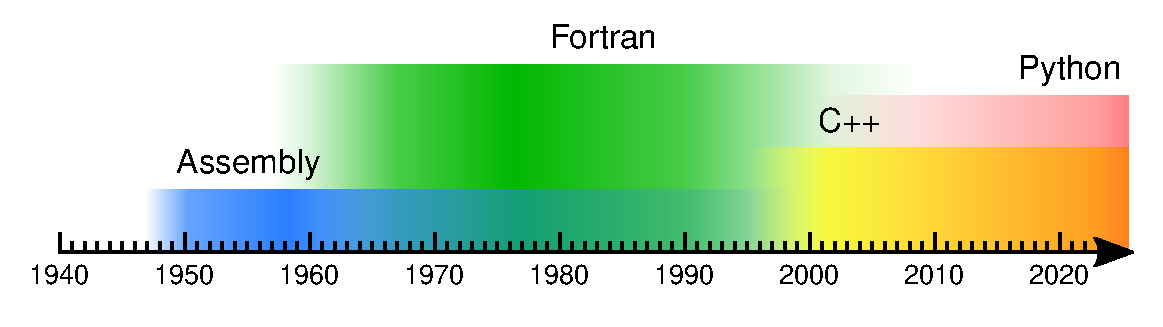
\includegraphics[width=\linewidth]{PLOTS/programming-languages.pdf}
%% \end{columns}

%% \large
%% \vspace{0.5 cm}
%% Adoption of

%% \begin{description}
%% \item[\textcolor{black}{Fortran:}] \textcolor{darkblue}{immediate;} \textcolor{darkgreen}{for syntax and portability;} \textcolor{violet}{no infrastructure to replace}
%% \item[\textcolor{black}{C++:}] \textcolor{darkblue}{long overdue;} \textcolor{darkgreen}{for data structures;} \textcolor{violet}{replaced infrastructure in a burst}
%% \item[\textcolor{black}{Python:}] \textcolor{darkblue}{slowly overtook its alternatives;} \textcolor{darkgreen}{for interactivity;} \textcolor{violet}{different niche}
%% \end{description}
%% \end{frame}

%% \begin{frame}{\mbox{ }}
%% \LARGE
%% \begin{center}
%% \textcolor{darkblue}{Part 1: Fortran}
%% \end{center}
%% \end{frame}

%% \begin{frame}{NHEP was an early adopter of digital computers}
%% \Large
%% \vspace{0.35 cm}
%% \begin{columns}
%% \column{1.05\linewidth}
%% One of the very first applications was Monte Carlo (neutron transport).

%% \vspace{-0.2 cm}
%% \begin{center}
%% 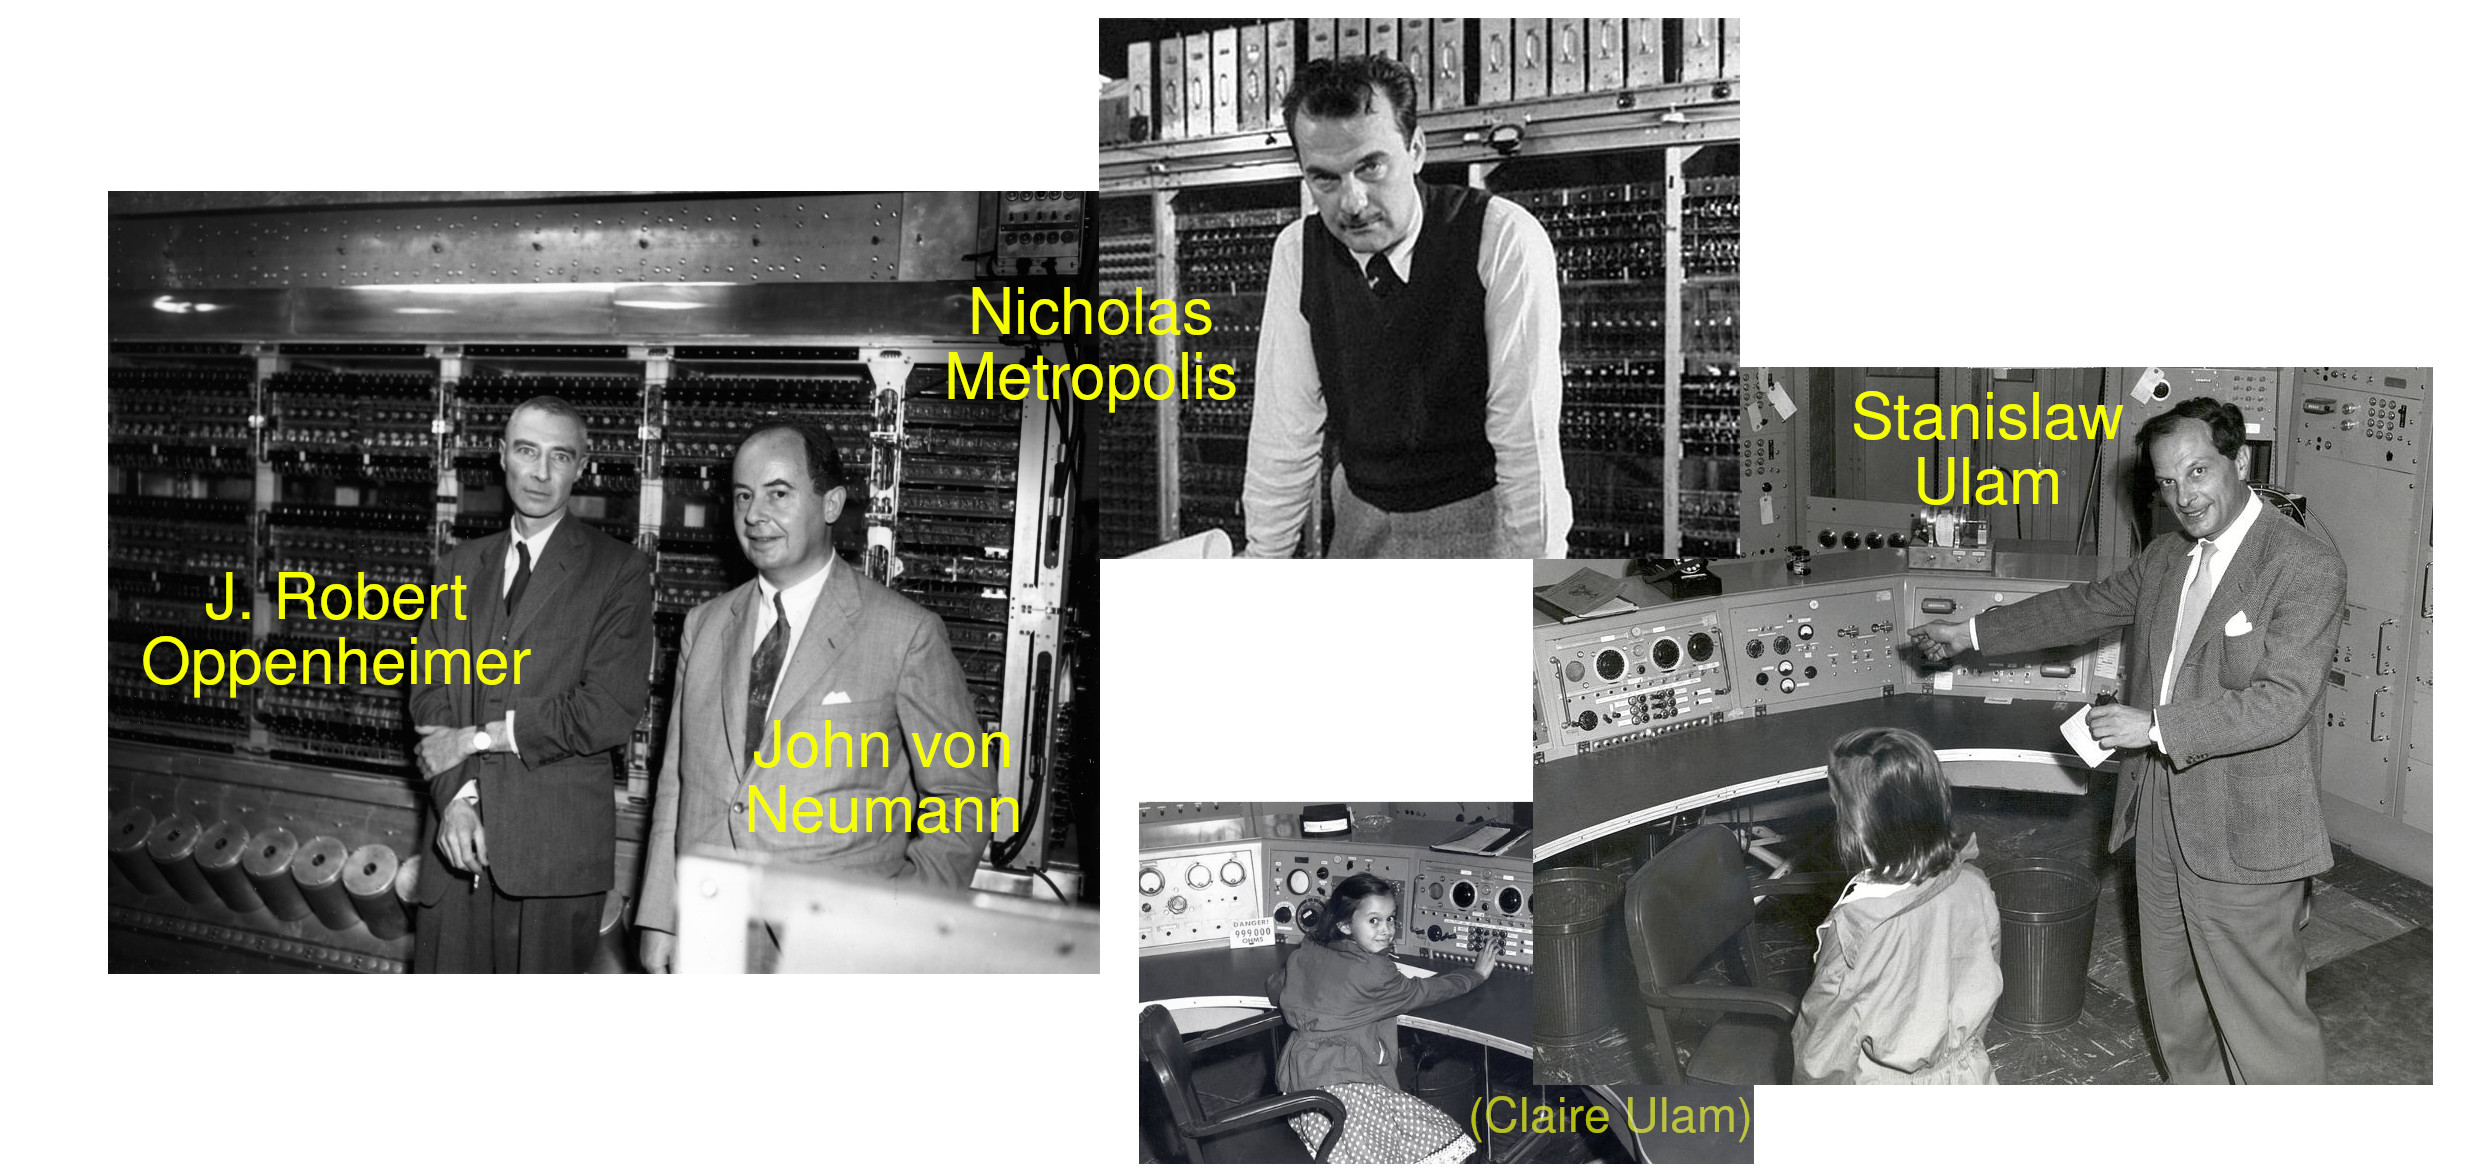
\includegraphics[width=\linewidth]{PLOTS/manhattan-project-physicists-and-computer.jpg}
%% \end{center}
%% \end{columns}
%% \end{frame}

%% \begin{frame}{And so was data analysis}
%% \large
%% \vspace{0.5 cm}
%% Luis Alvarez's group at the Bevatron: \textcolor{darkgreen}{\$2M} bubble chamber, \textcolor{darkgreen}{\$0.2M} IBM 650.

%% \vspace{0.5 cm}
%% 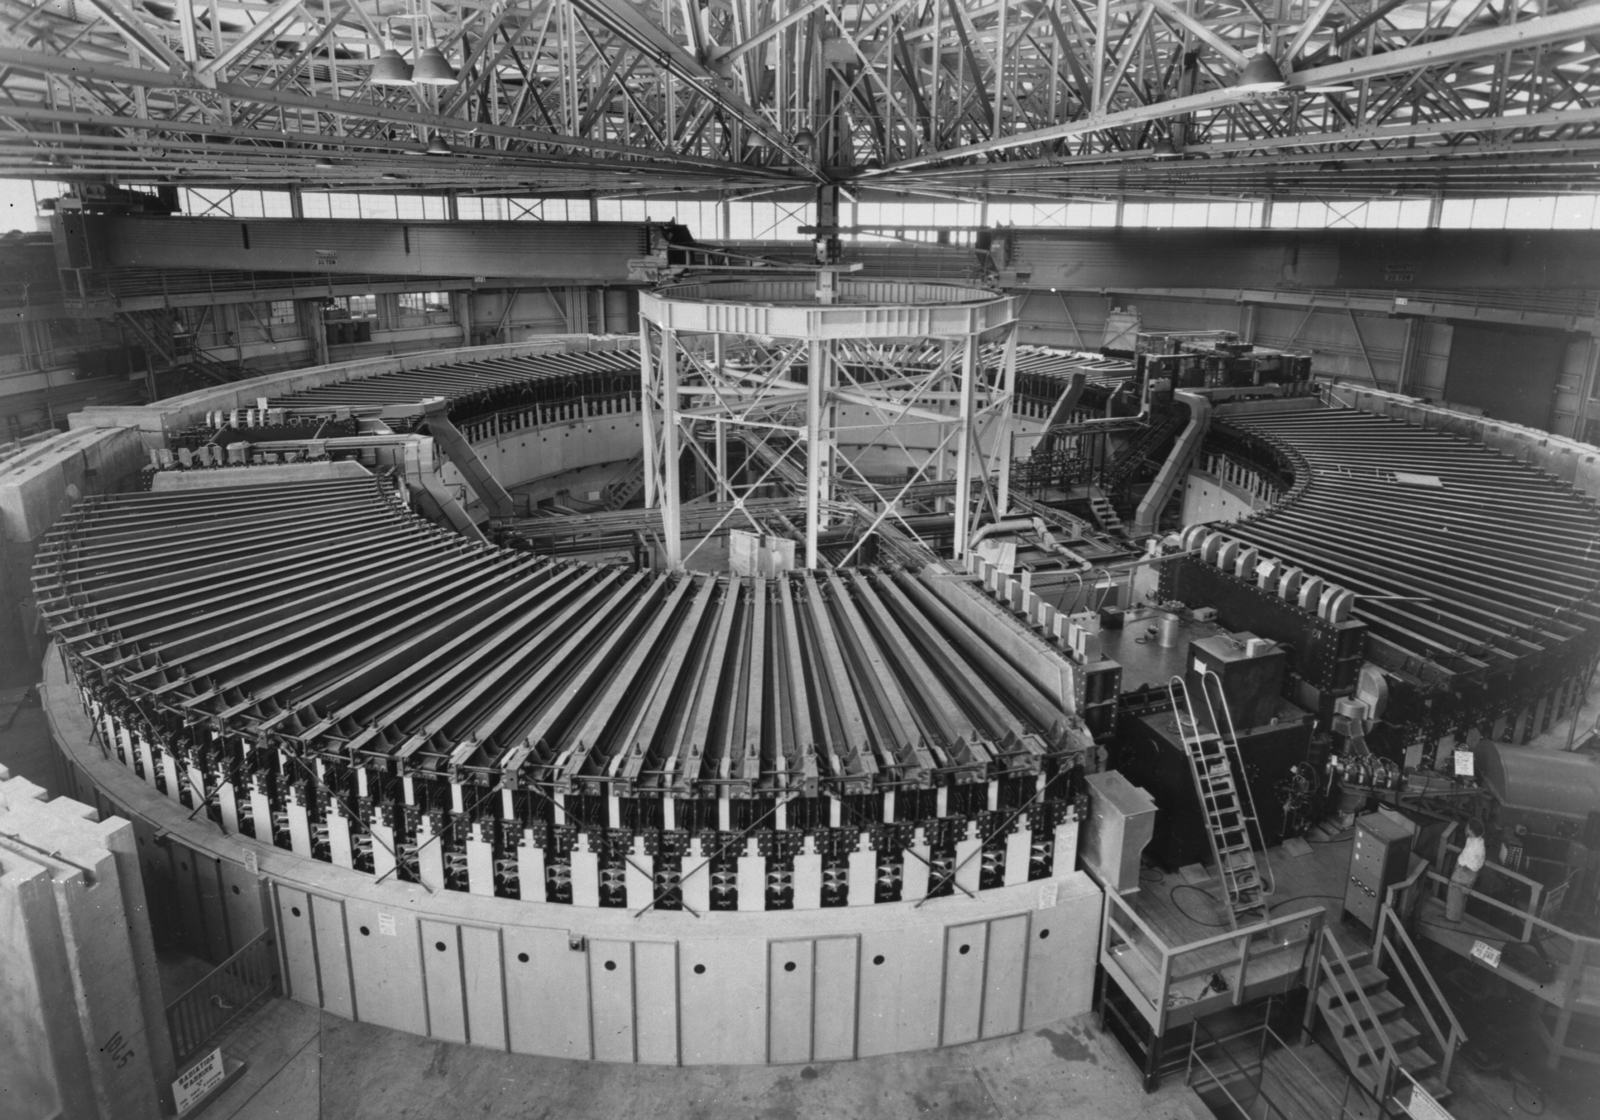
\includegraphics[width=0.45\linewidth]{PLOTS/overall-view-of-bevatron-magnet-photograph-taken-september-6-1955-bevatron-088cb0-1600.jpg}\hfill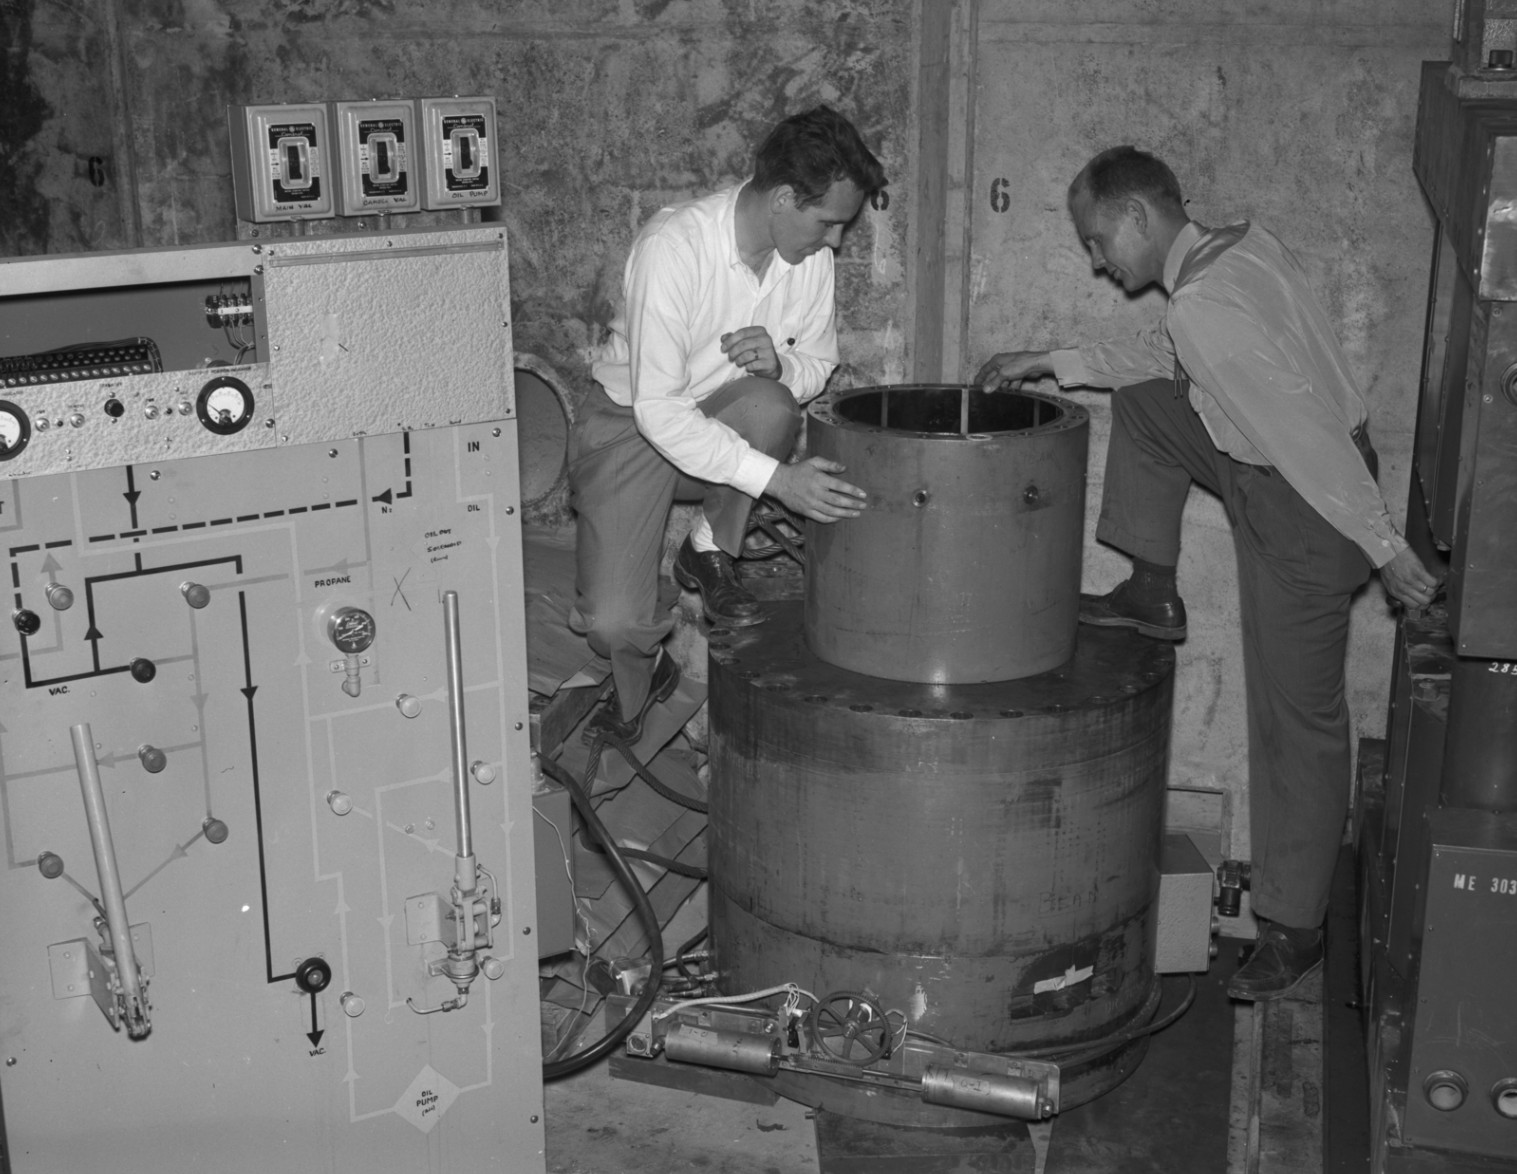
\includegraphics[width=0.5\linewidth]{PLOTS/alvarez-group-bubble-chamber.jpg}
%% \end{frame}

%% \begin{frame}{The problem was the same then as it is now}
%% \vspace{0.4 cm}
%% \begin{columns}
%% \column{0.25\linewidth}
%% \only<1>{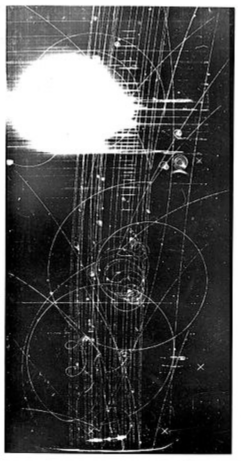
\includegraphics[height=7.5 cm]{PLOTS/bubble-chamber-photo-0.pdf}}\only<2->{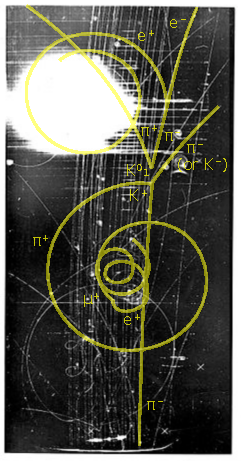
\includegraphics[height=7.5 cm]{PLOTS/bubble-chamber-photo.pdf}}

%% \column{0.2\linewidth}
%% Unlabeled photos come out of the detector.

%% \vspace{0.5 cm}
%% \uncover<2->{Labeling them turns them into quantities to compute.}

%% \vspace{0.5 cm}
%% \uncover<3->{THE MORE EVENTS THE BETTER!!!}

%% \column{0.4\linewidth}
%% \uncover<3->{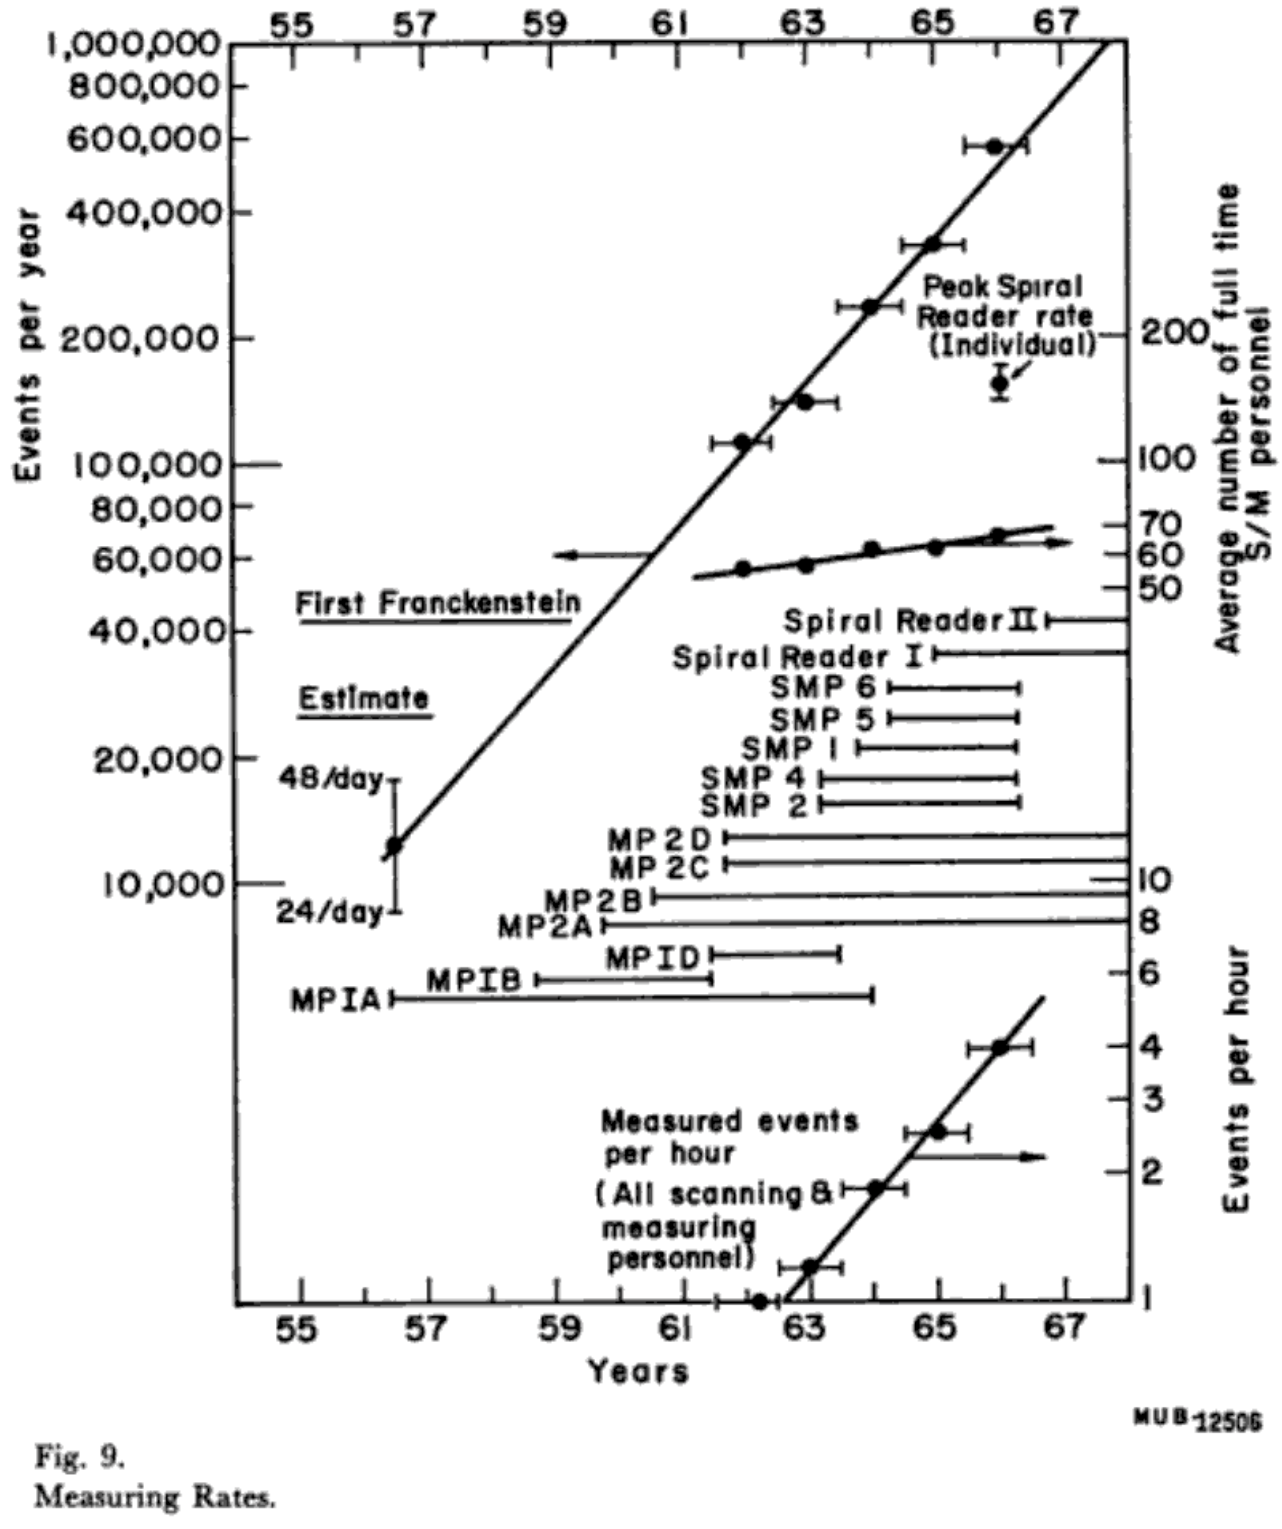
\includegraphics[height=7.5 cm]{PLOTS/scaleup.png}}
%% \end{columns}
%% \end{frame}

%% \begin{frame}{The problem was the same then as it is now}
%% \vspace{0.25 cm}
%% \begin{columns}
%% \column{1.1\linewidth}
%% 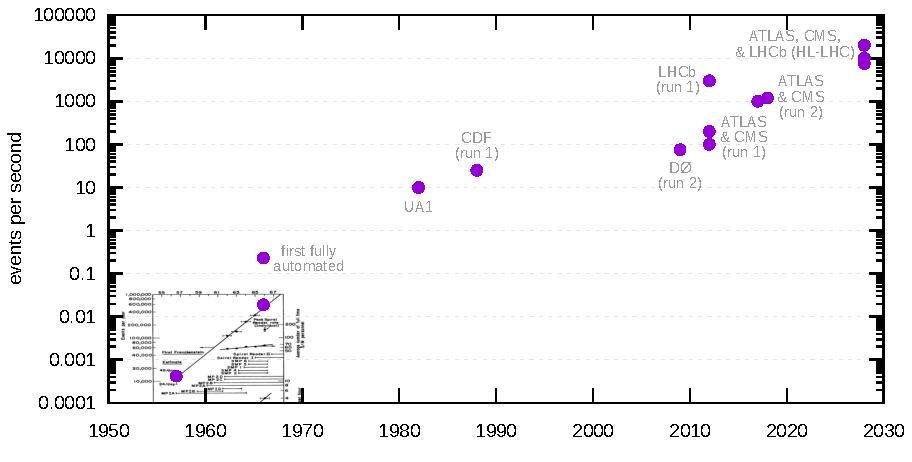
\includegraphics[width=\linewidth]{PLOTS/event-rates.pdf}
%% \end{columns}
%% \end{frame}

%% \begin{frame}{Identifying tracks was beyond the capabilities of software}
%% \Large
%% \vspace{0.35 cm}
%% \begin{columns}
%% \column{0.7\linewidth}
%% 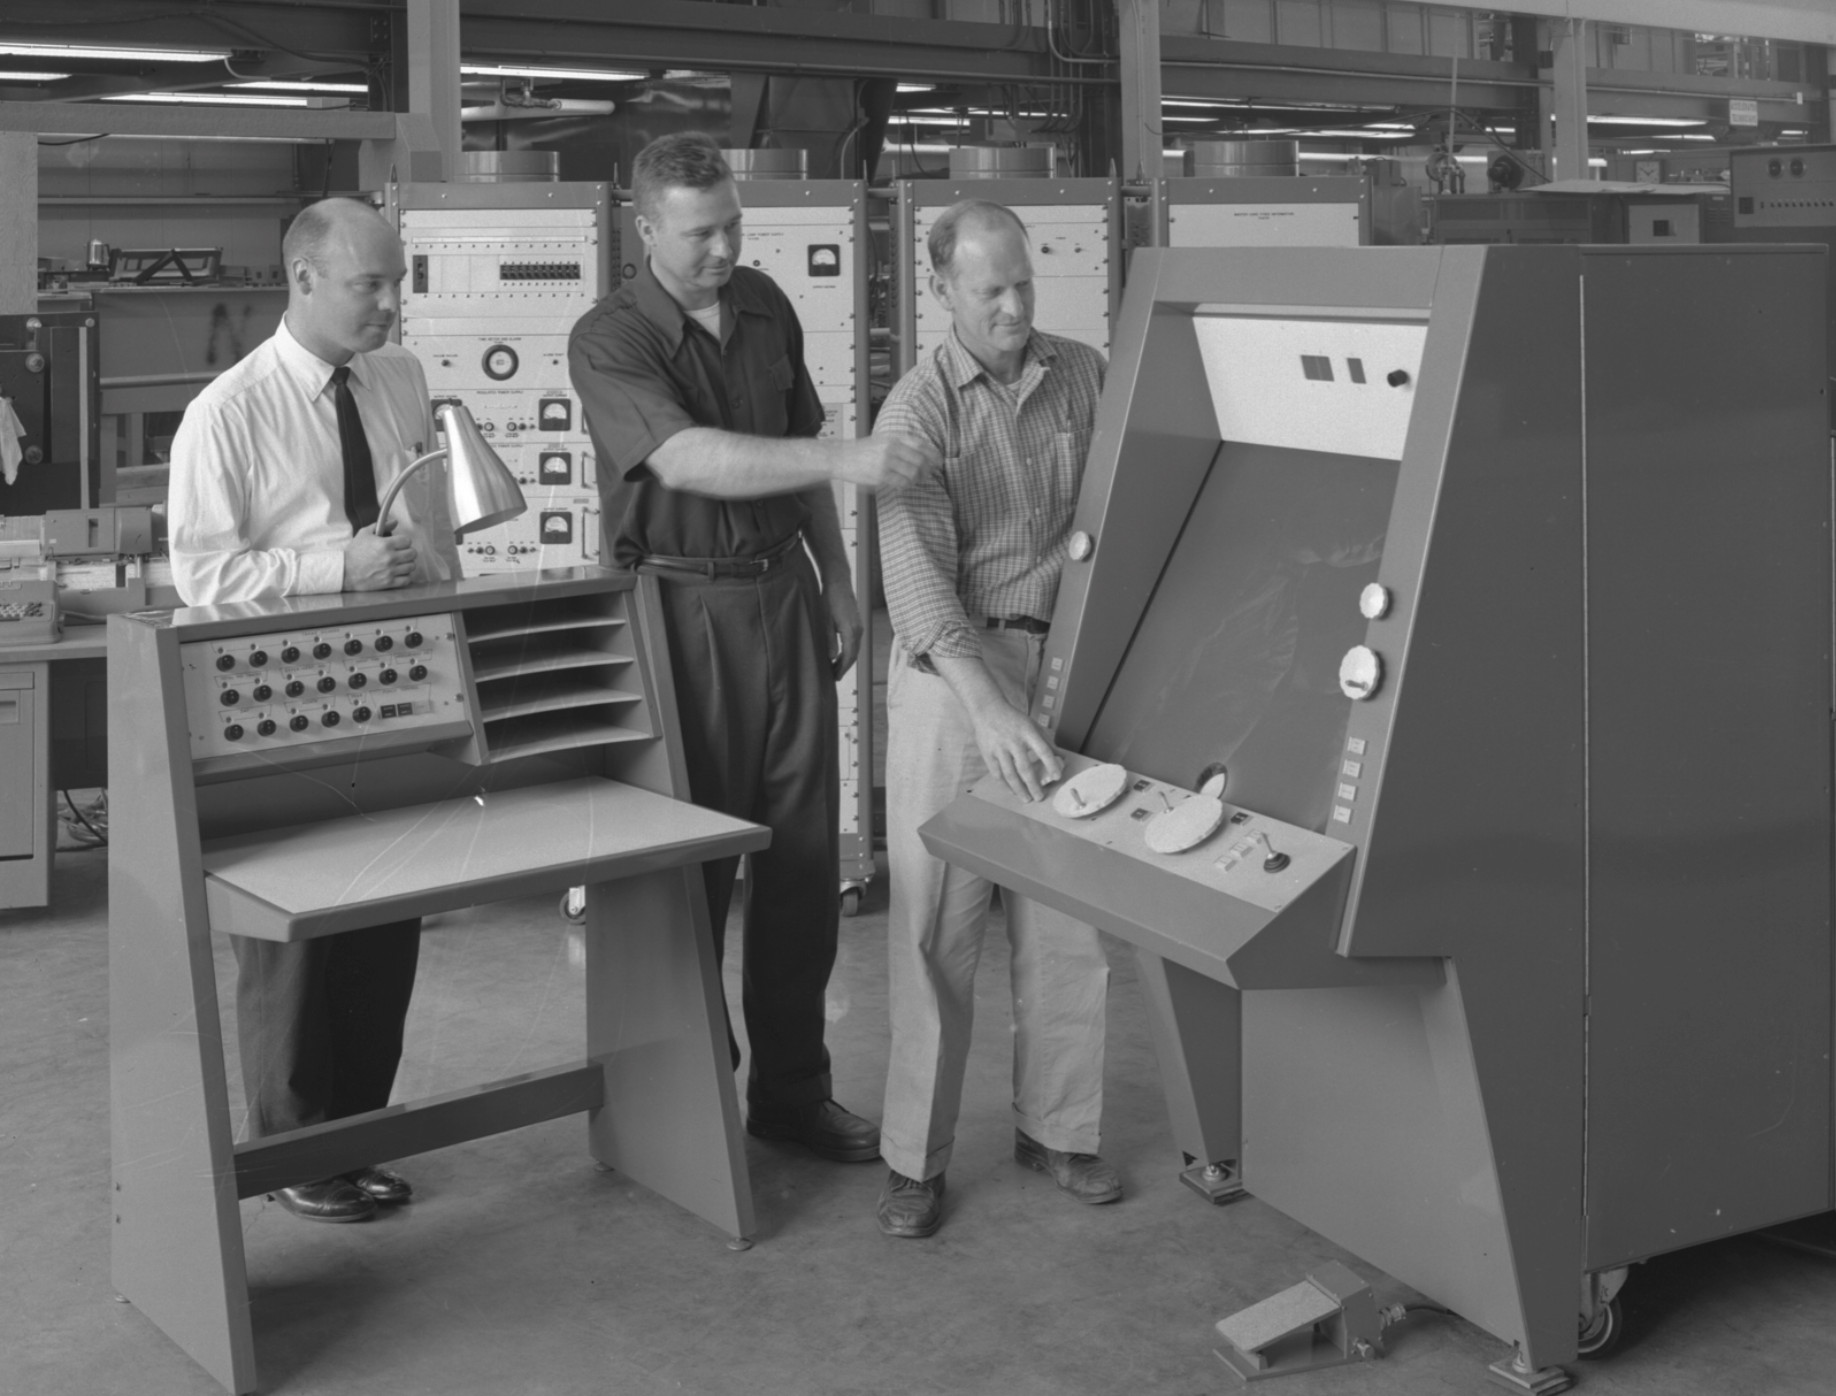
\includegraphics[width=\linewidth]{PLOTS/franckenstein-2.jpg}

%% \column{0.3\linewidth}
%% So they invented special input devices to streamline data-entry.

%% \end{columns}
%% \end{frame}

%% \begin{frame}{Identifying tracks was beyond the capabilities of software}
%% \vspace{0.35 cm}
%% \begin{columns}
%% \column{0.7\linewidth}
%% \only<1>{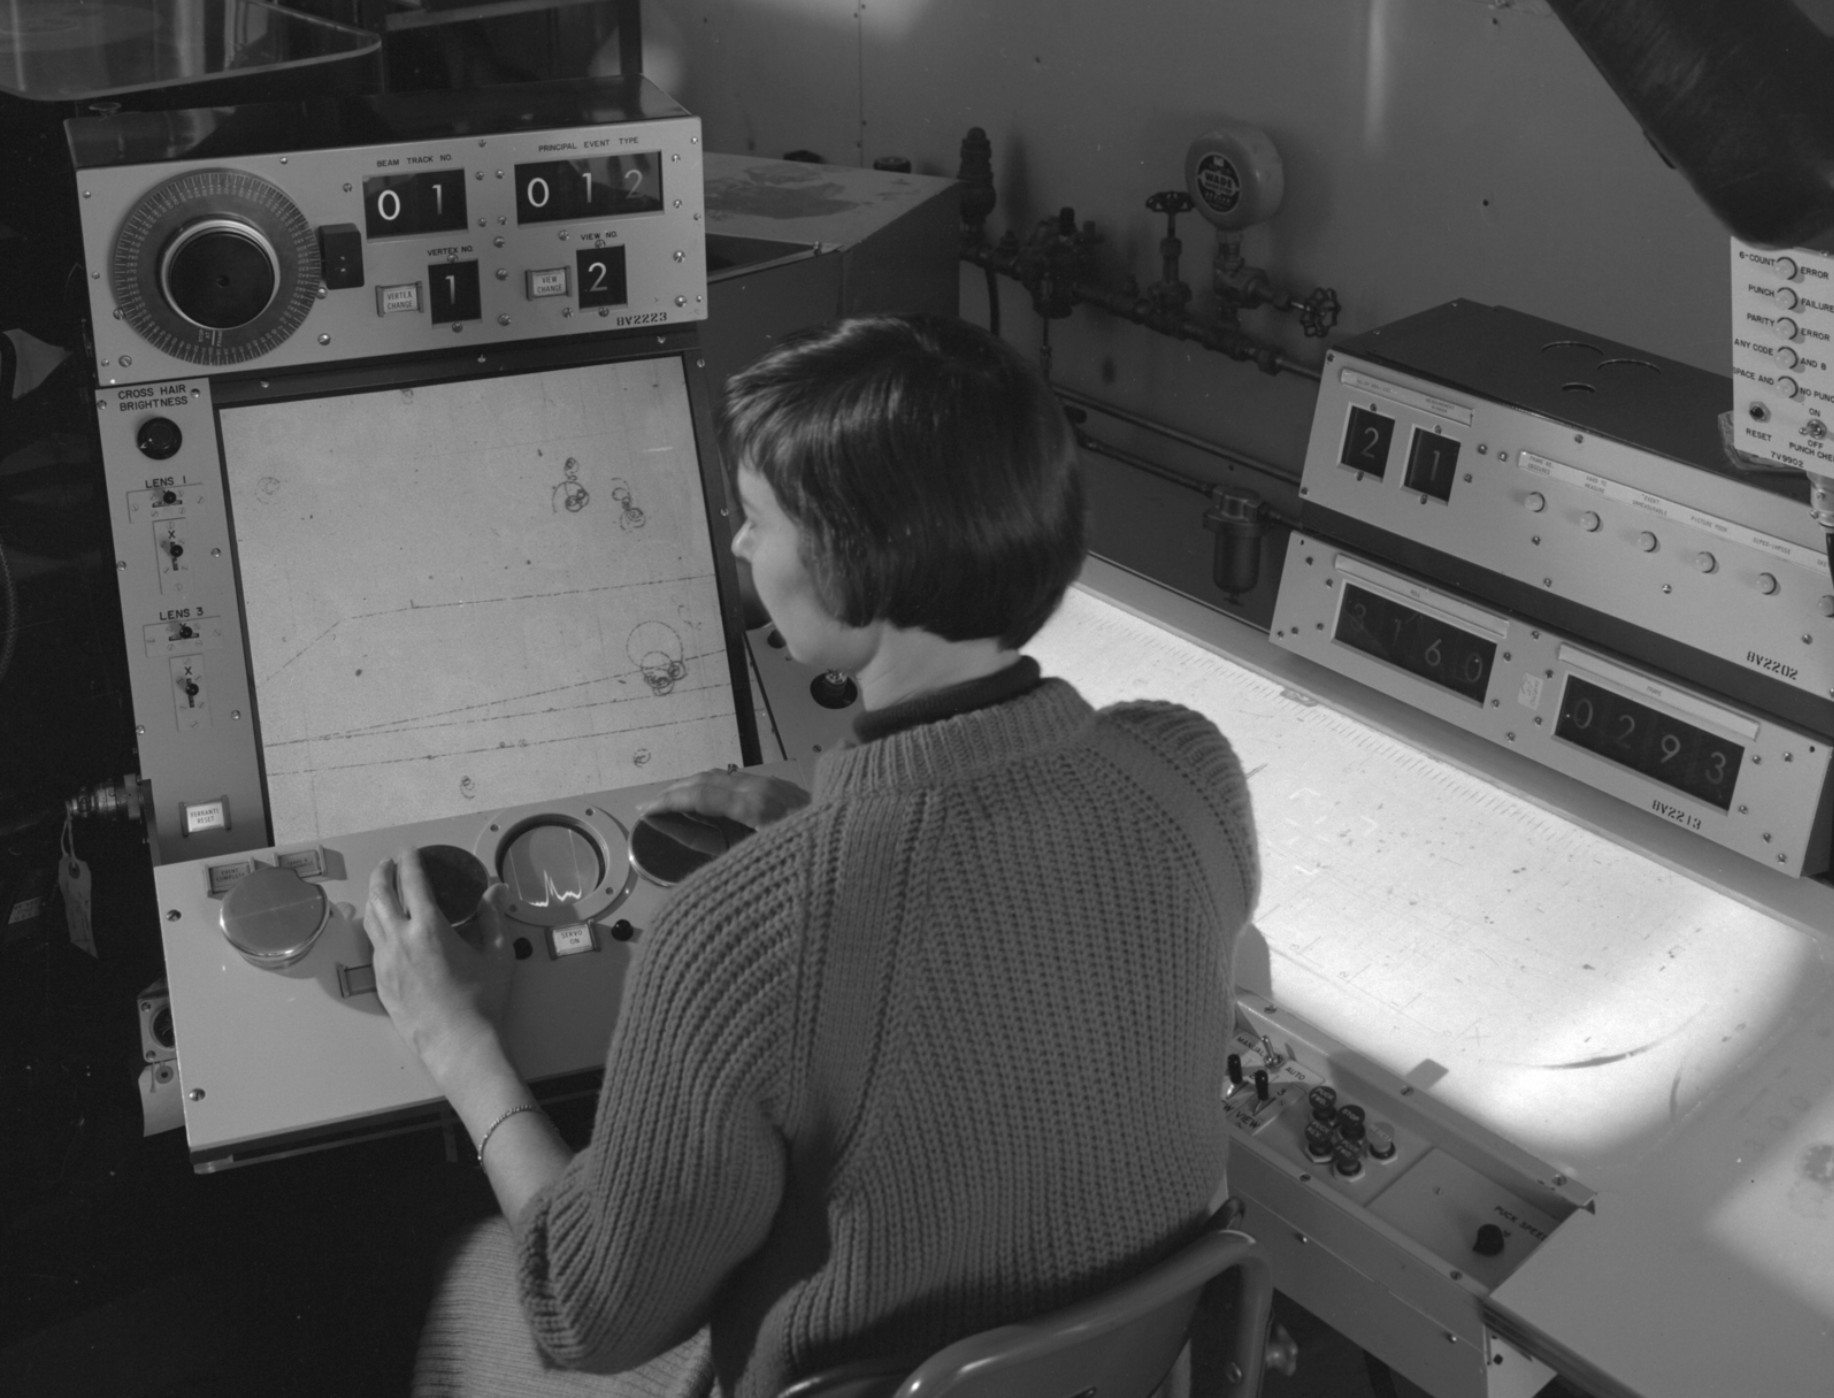
\includegraphics[width=\linewidth]{PLOTS/franckenstein-3.jpg}}\only<2>{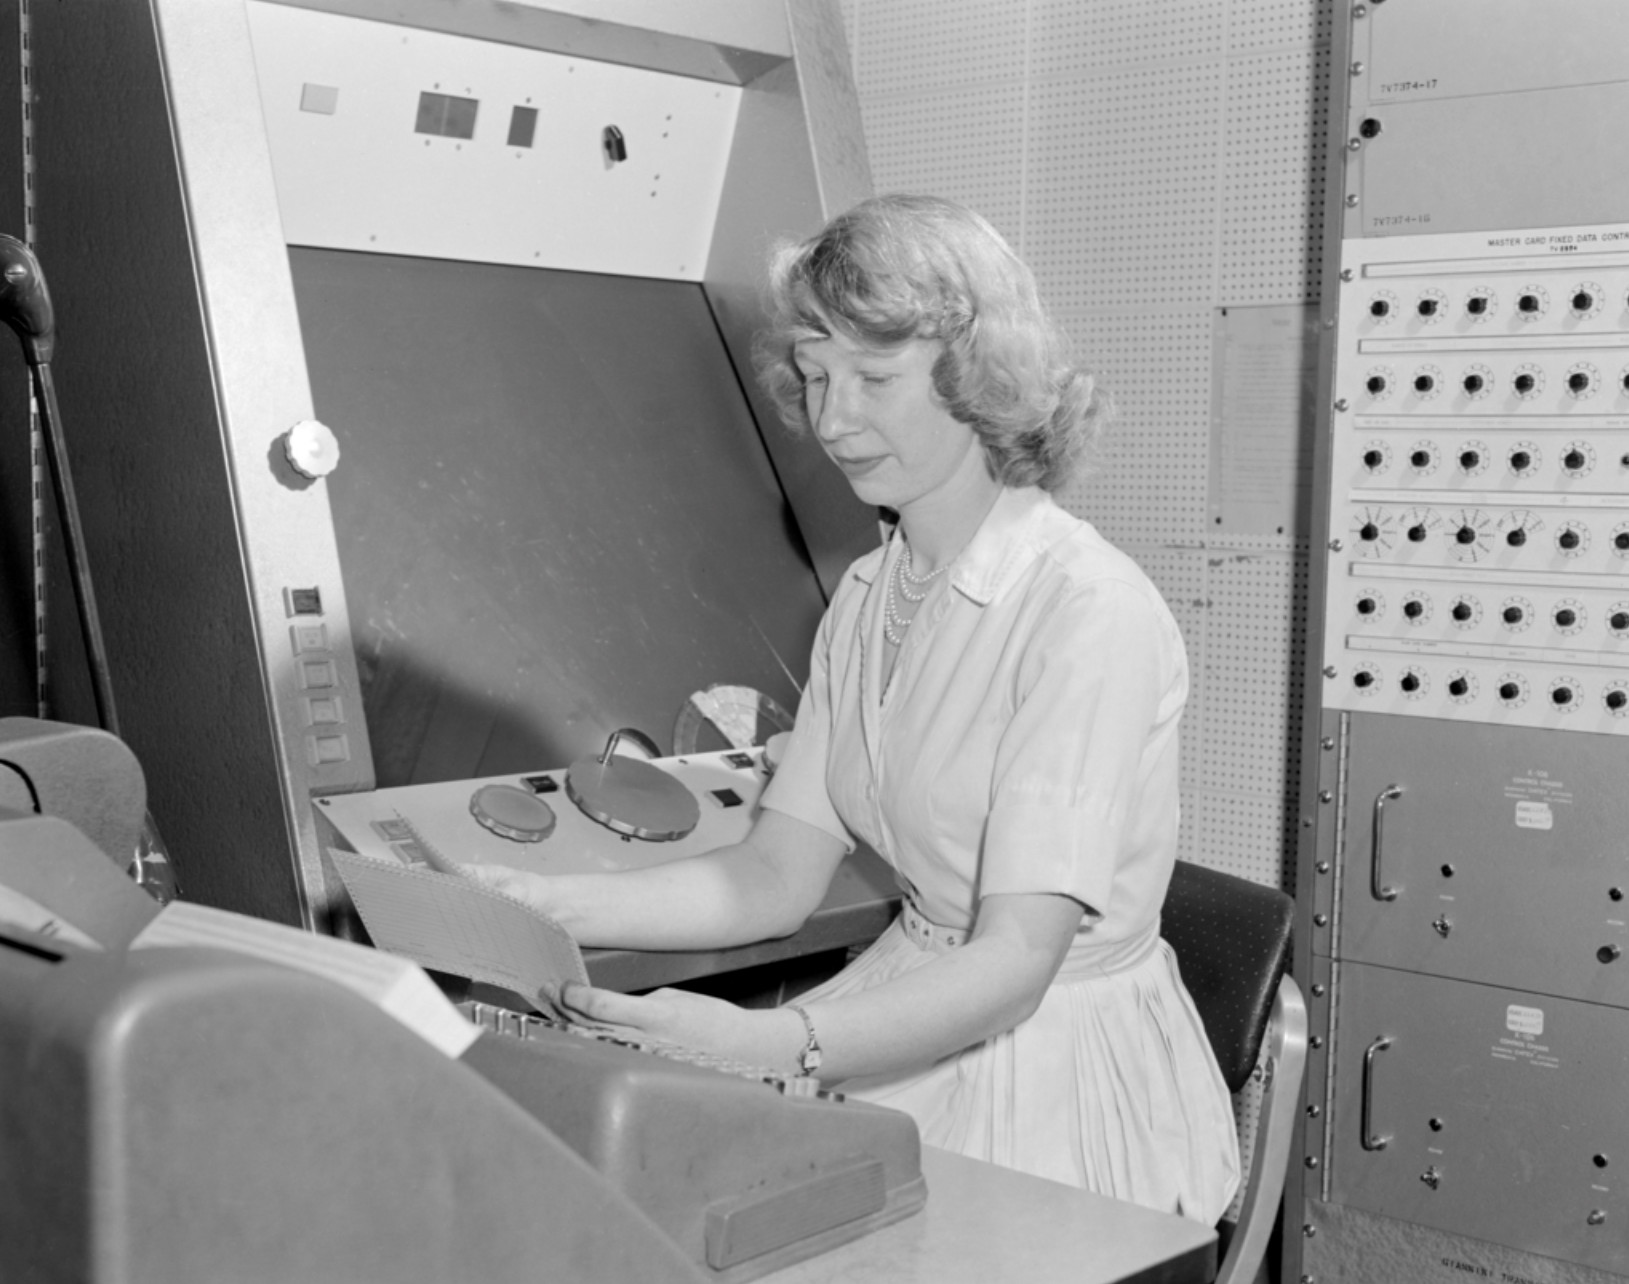
\includegraphics[width=\linewidth]{PLOTS/franckenstein-4.jpg}}

%% \column{0.3\linewidth}
%% \only<1>{\vspace{-0.5 cm}}\only<2>{\vspace{-1.25 cm}}
%% \begin{center}
%% 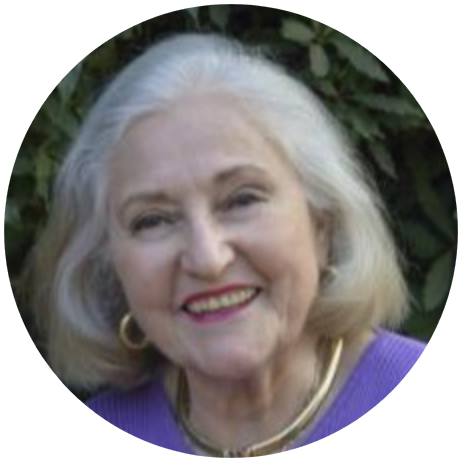
\includegraphics[width=0.5\linewidth]{PLOTS/madeleine-isenberg-SCANNER.png}

%% \scriptsize
%% Madeleine (n\'ee Goldstein) Isenberg, UCLA class of '65
%% \end{center}

%% \begin{minipage}{\linewidth}
%% \scriptsize
%% \begin{onlyenv}<1>
%% ``We scanners would review each frame of film, and per the brief instructions we had been given, looked for any `unusual activity.'

%% \vspace{0.25 cm}
%% ``The scanner had to use both hands, a joystick in each, and turn them clockwise or anti-clockwise, to align a double crosshair cursor at several sequential positions on a track.''
%% \end{onlyenv}\begin{onlyenv}<2>
%% ``A quick but firm tap on the foot-pedal punched the coordinate values onto an IBM card that had been fed into the keypunch machine.

%% \vspace{0.25 cm}
%% ``The precious stack of IBM cards were passed to the physicists, who would then process the data in the existing IBM processors, using software that would calculate the best fit for these coordinates, and thereby mathematically simulate the curvature of the track.''
%% \end{onlyenv}
%% \end{minipage}
%% \end{columns}
%% \end{frame}

%% \begin{frame}{At first, the software was written in assembly (example from 1958)}
%% \vspace{0.25 cm}

%% 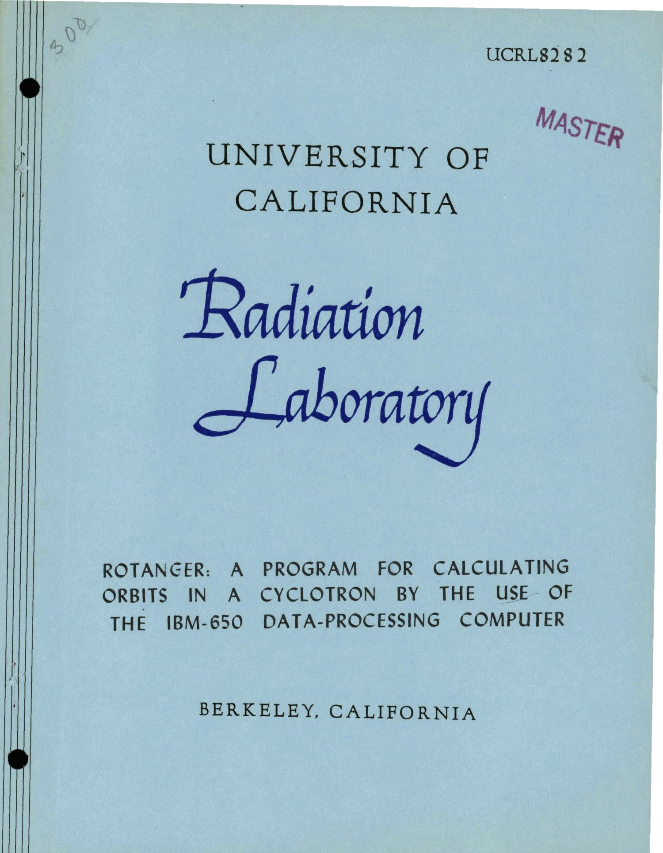
\includegraphics[height=7 cm]{PLOTS/assembly-language-program-berkeley.png}

%% \vspace{-6.9 cm}
%% \uncover<2->{\mbox{\hspace{1.8 cm}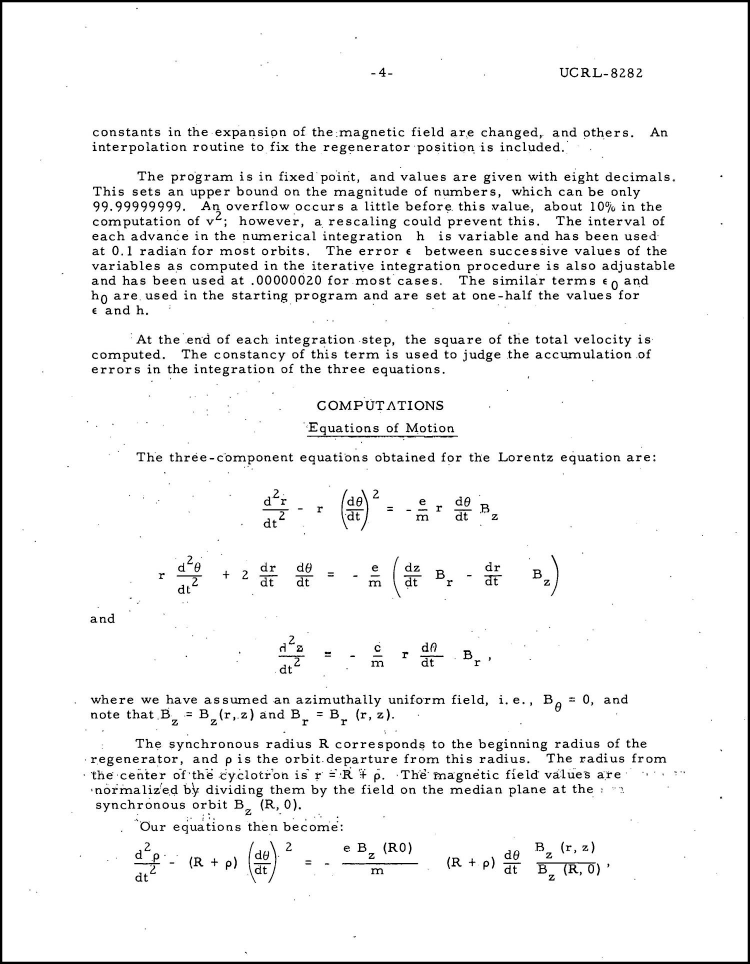
\includegraphics[height=7 cm]{PLOTS/assembly-language-program-berkeley-1.png}}}

%% \vspace{-6.9 cm}
%% \uncover<3->{\mbox{\hspace{3.6 cm}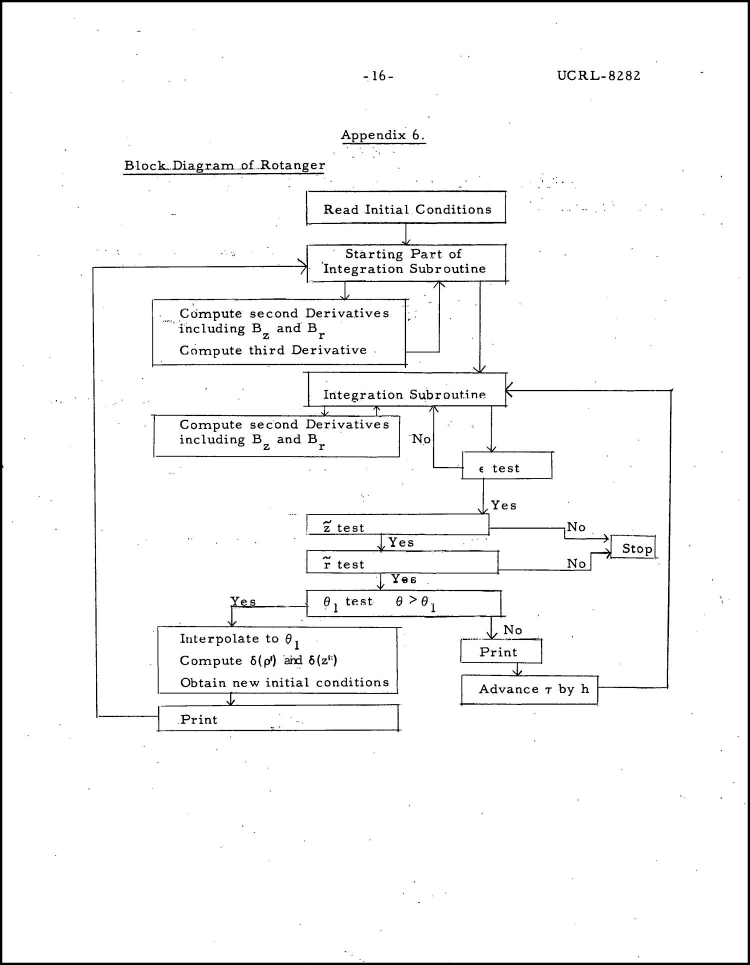
\includegraphics[height=7 cm]{PLOTS/assembly-language-program-berkeley-2.png}}}

%% \vspace{-6.9 cm}
%% \uncover<4->{\mbox{\hspace{5.4 cm}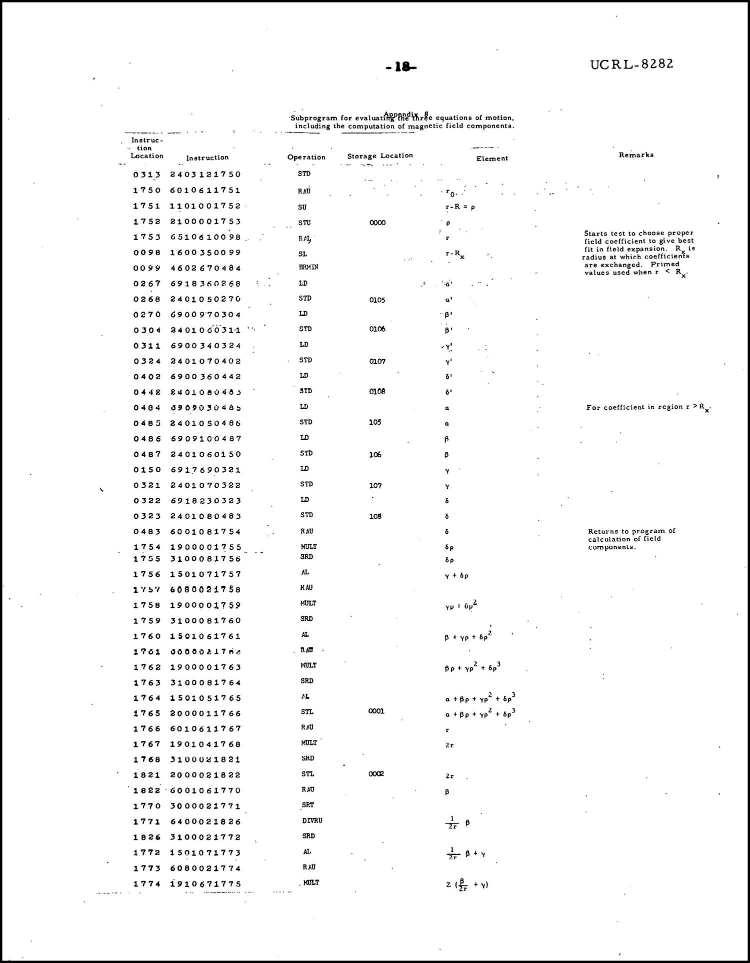
\includegraphics[height=7 cm]{PLOTS/assembly-language-program-berkeley-3.png}}}

%% \vspace{-6.9 cm}
%% \uncover<5->{\mbox{\hspace{7.2 cm}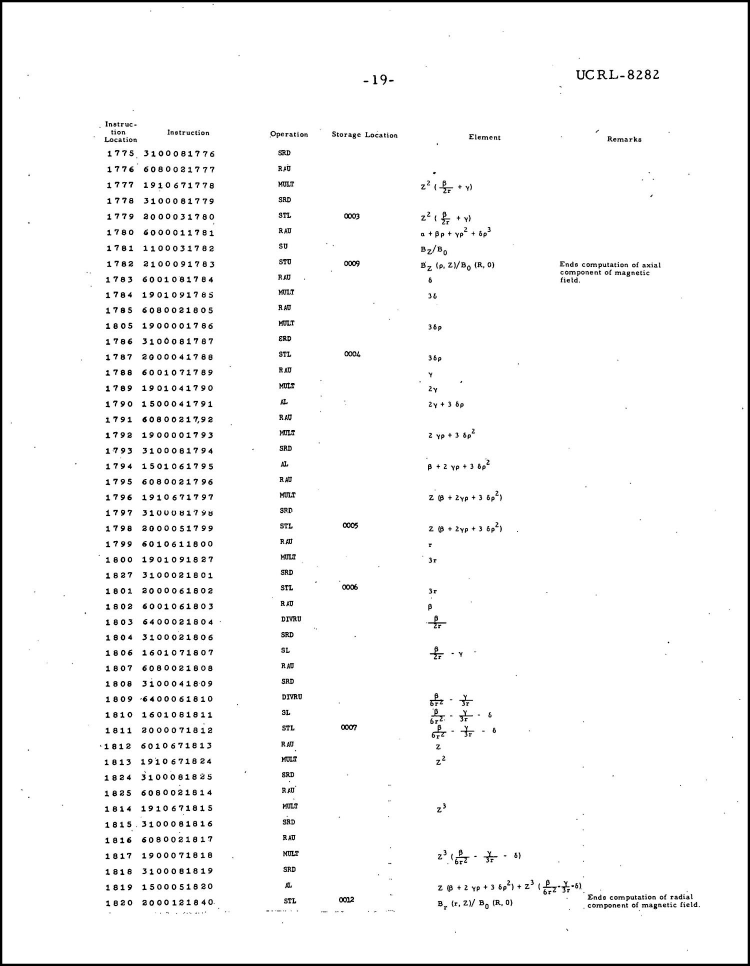
\includegraphics[height=7 cm]{PLOTS/assembly-language-program-berkeley-4.png}}}

%% \vspace{-6.9 cm}
%% \uncover<6->{\mbox{\hspace{9 cm}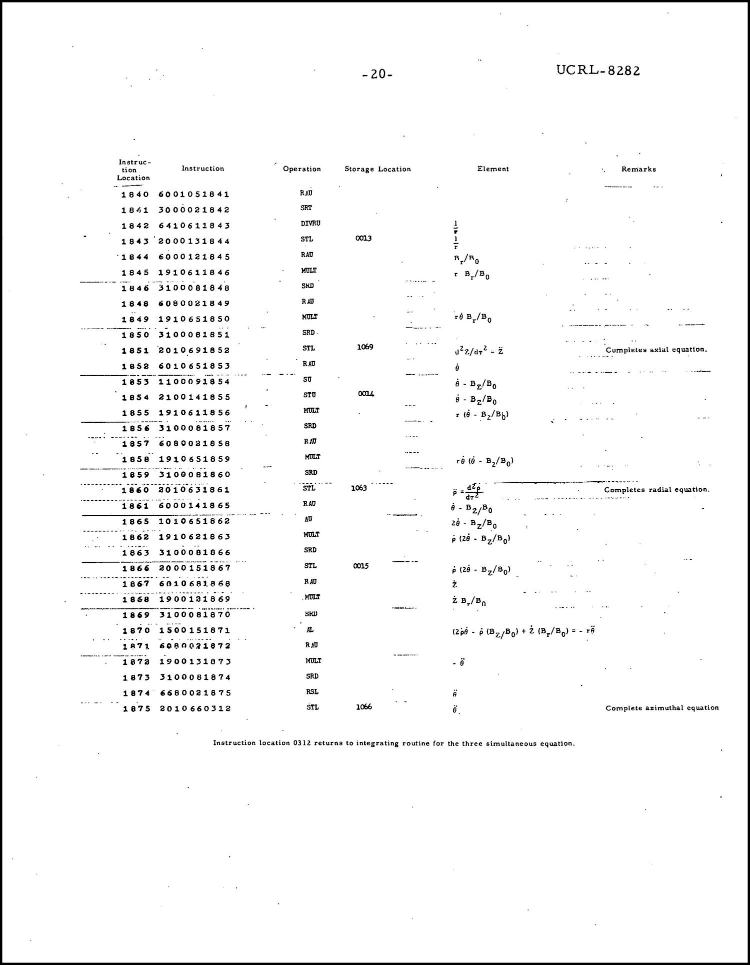
\includegraphics[height=7 cm]{PLOTS/assembly-language-program-berkeley-5.png}}}
%% \end{frame}

%% \begin{frame}{But it was quickly replaced by Fortran (example from 1964)}
%% \vspace{0.5 cm}
%% \begin{columns}
%% \column{1.1\linewidth}
%% 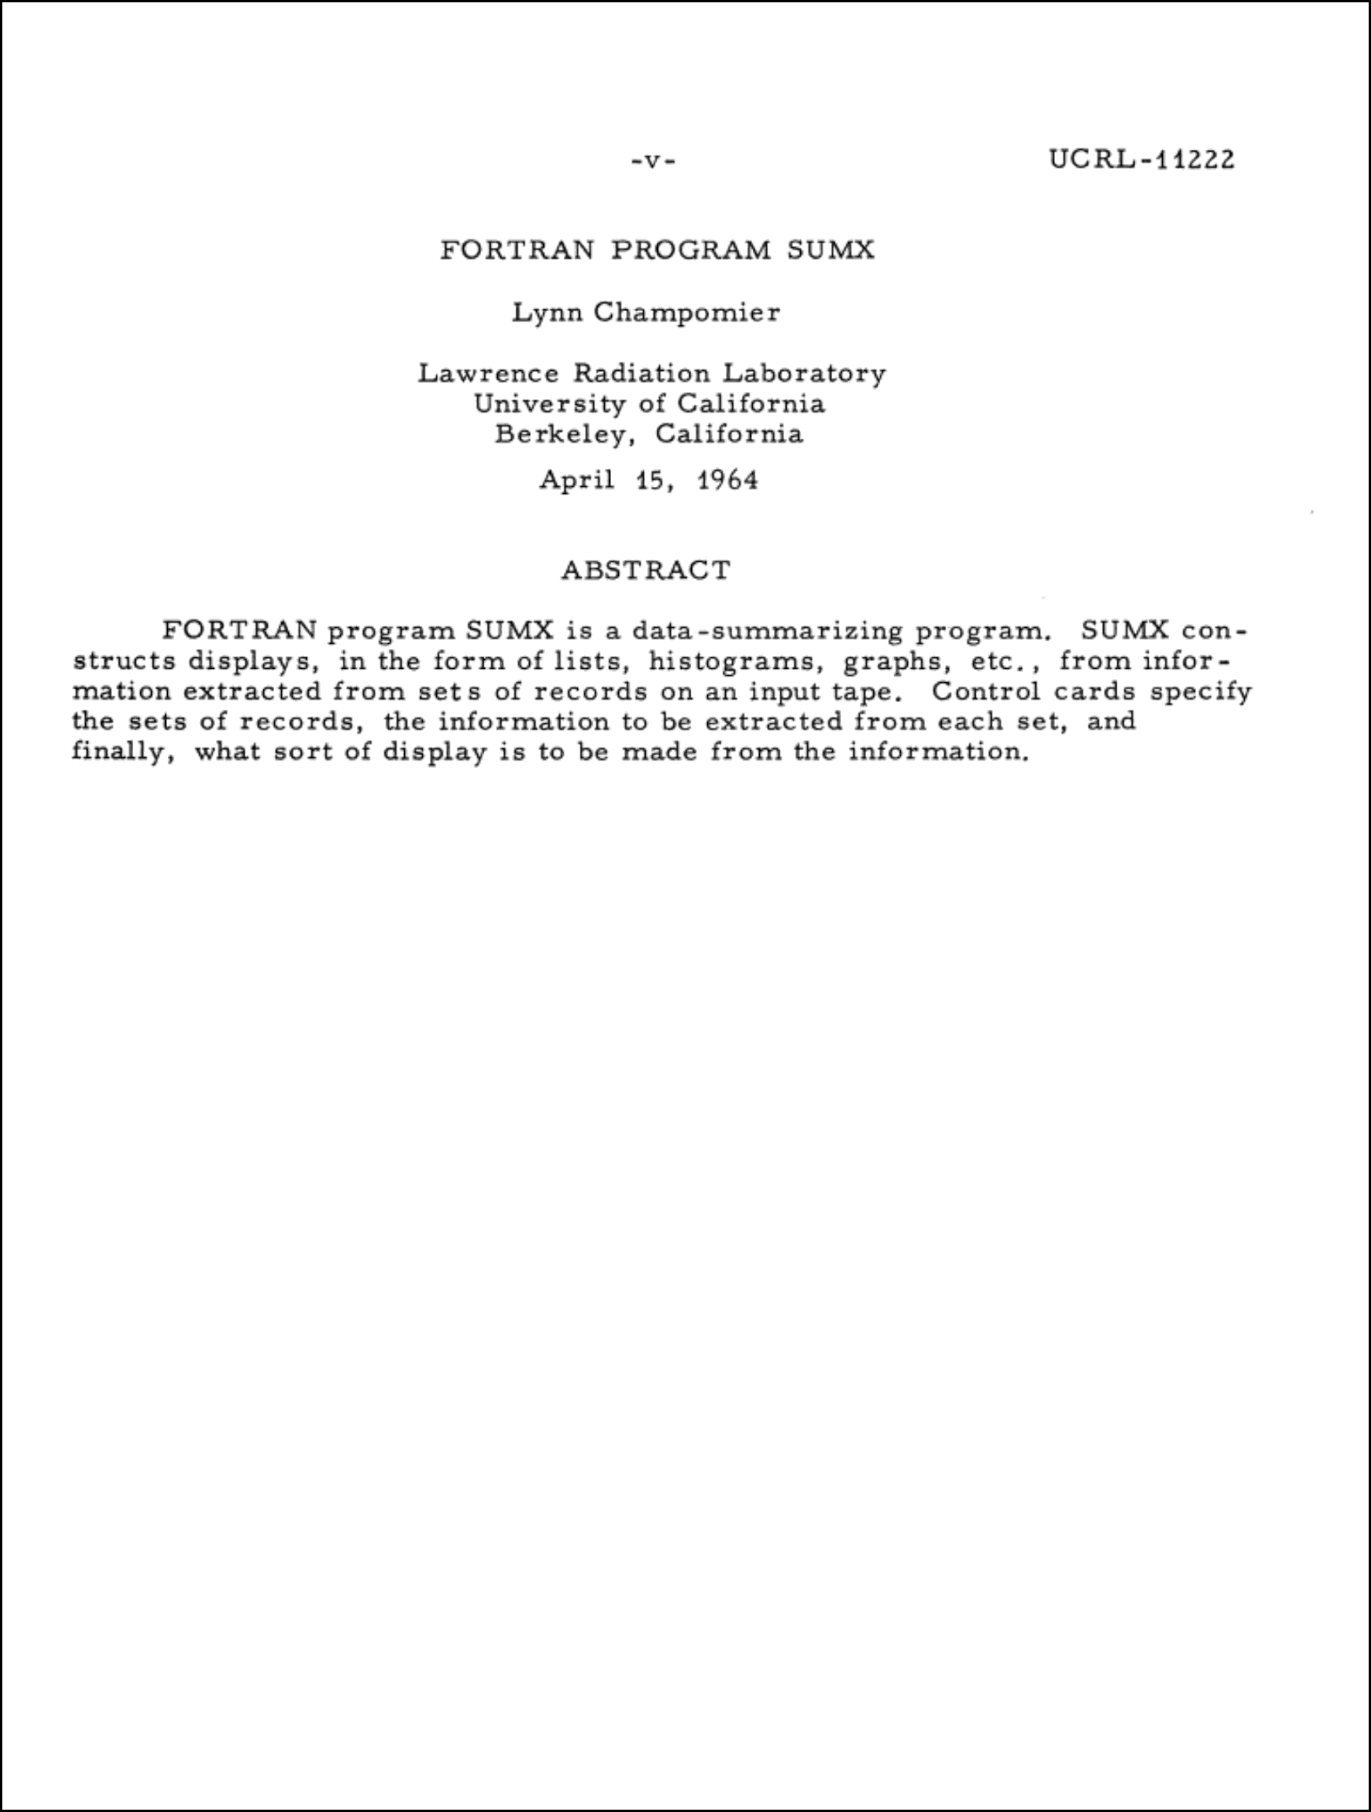
\includegraphics[height=6.5 cm]{PLOTS/sumx-cover.png}\hfill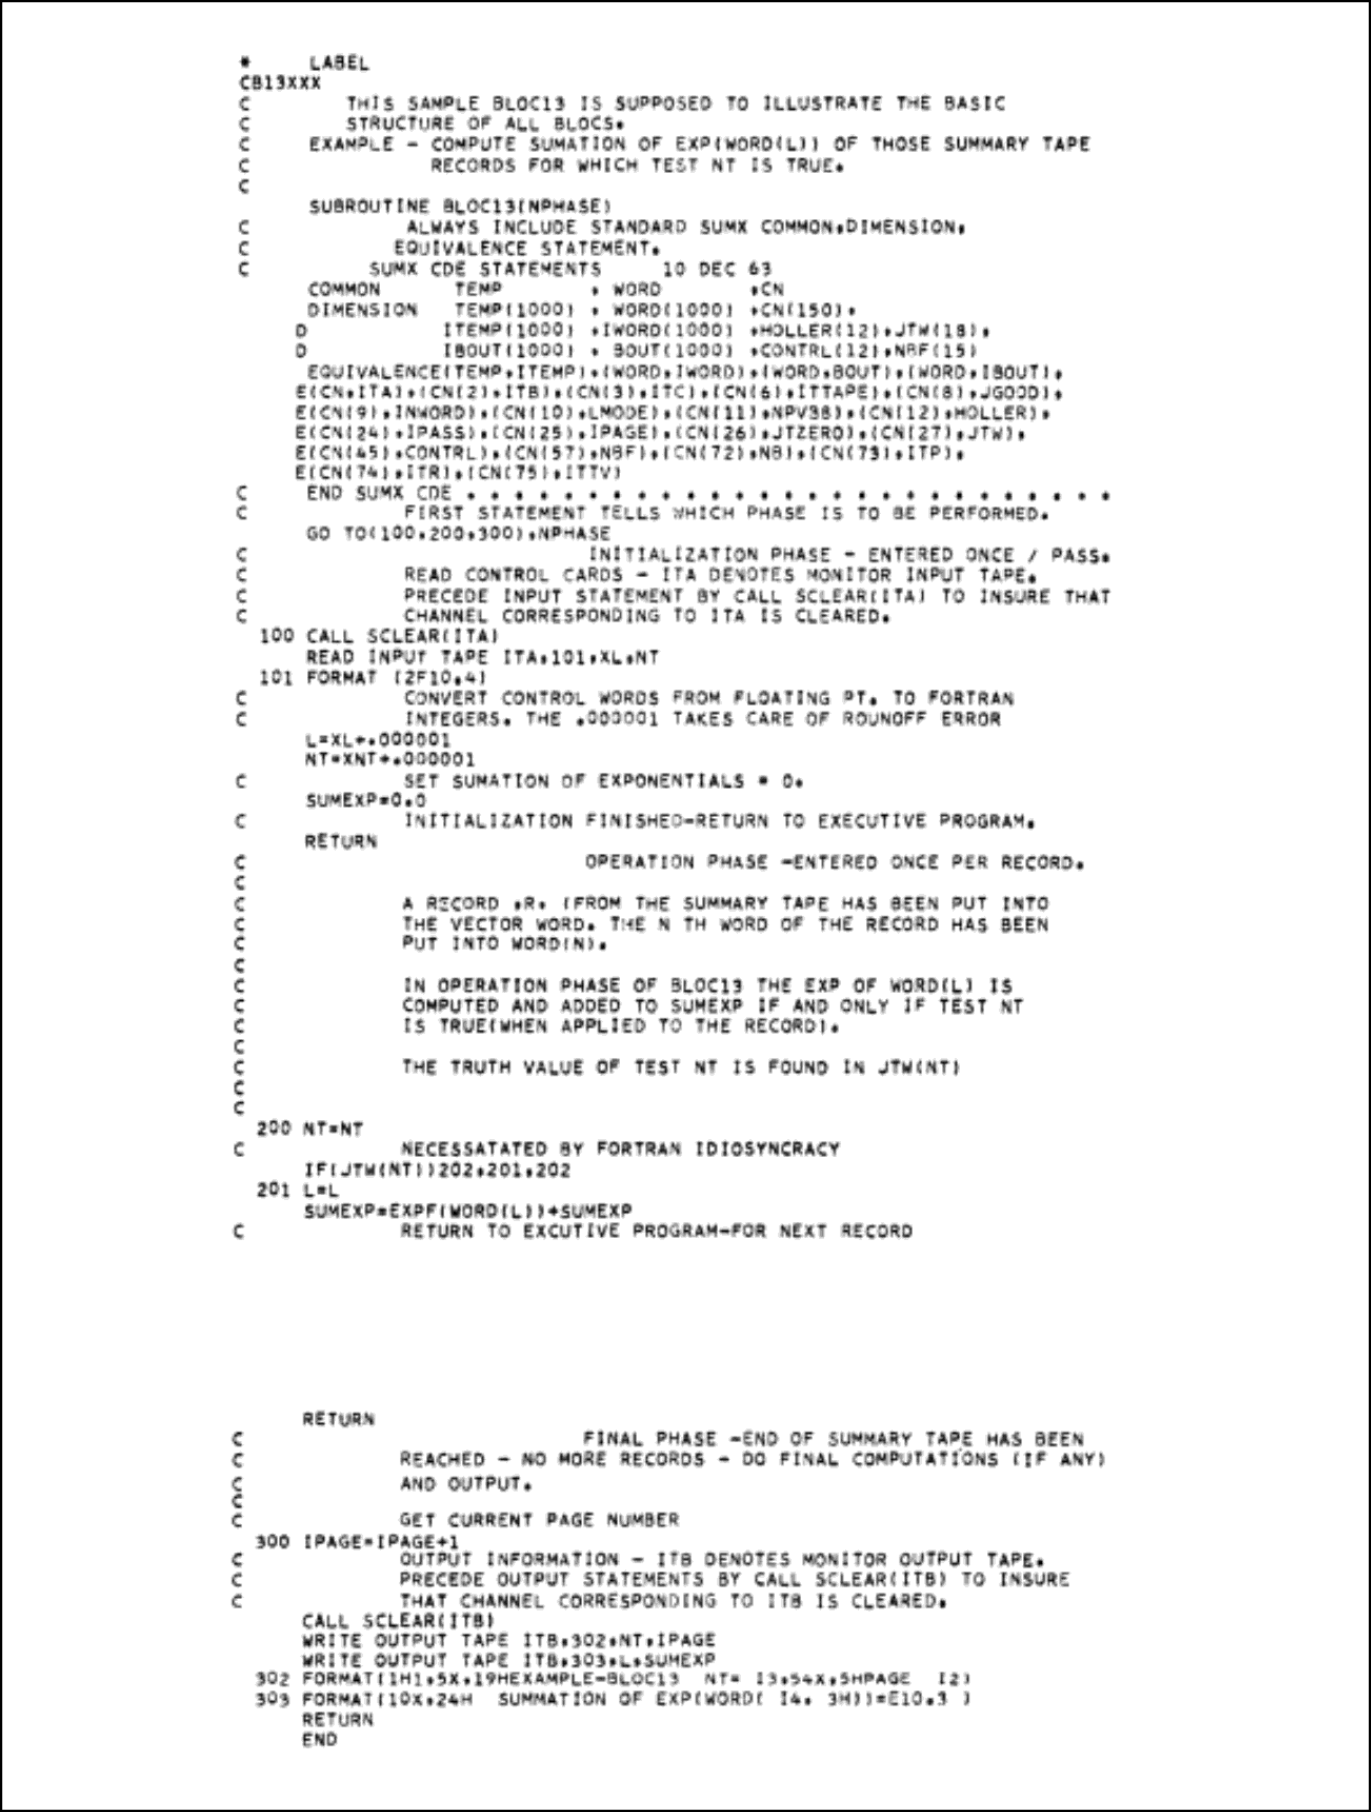
\includegraphics[height=6.5 cm]{PLOTS/sumx-code-sample.png}\hfill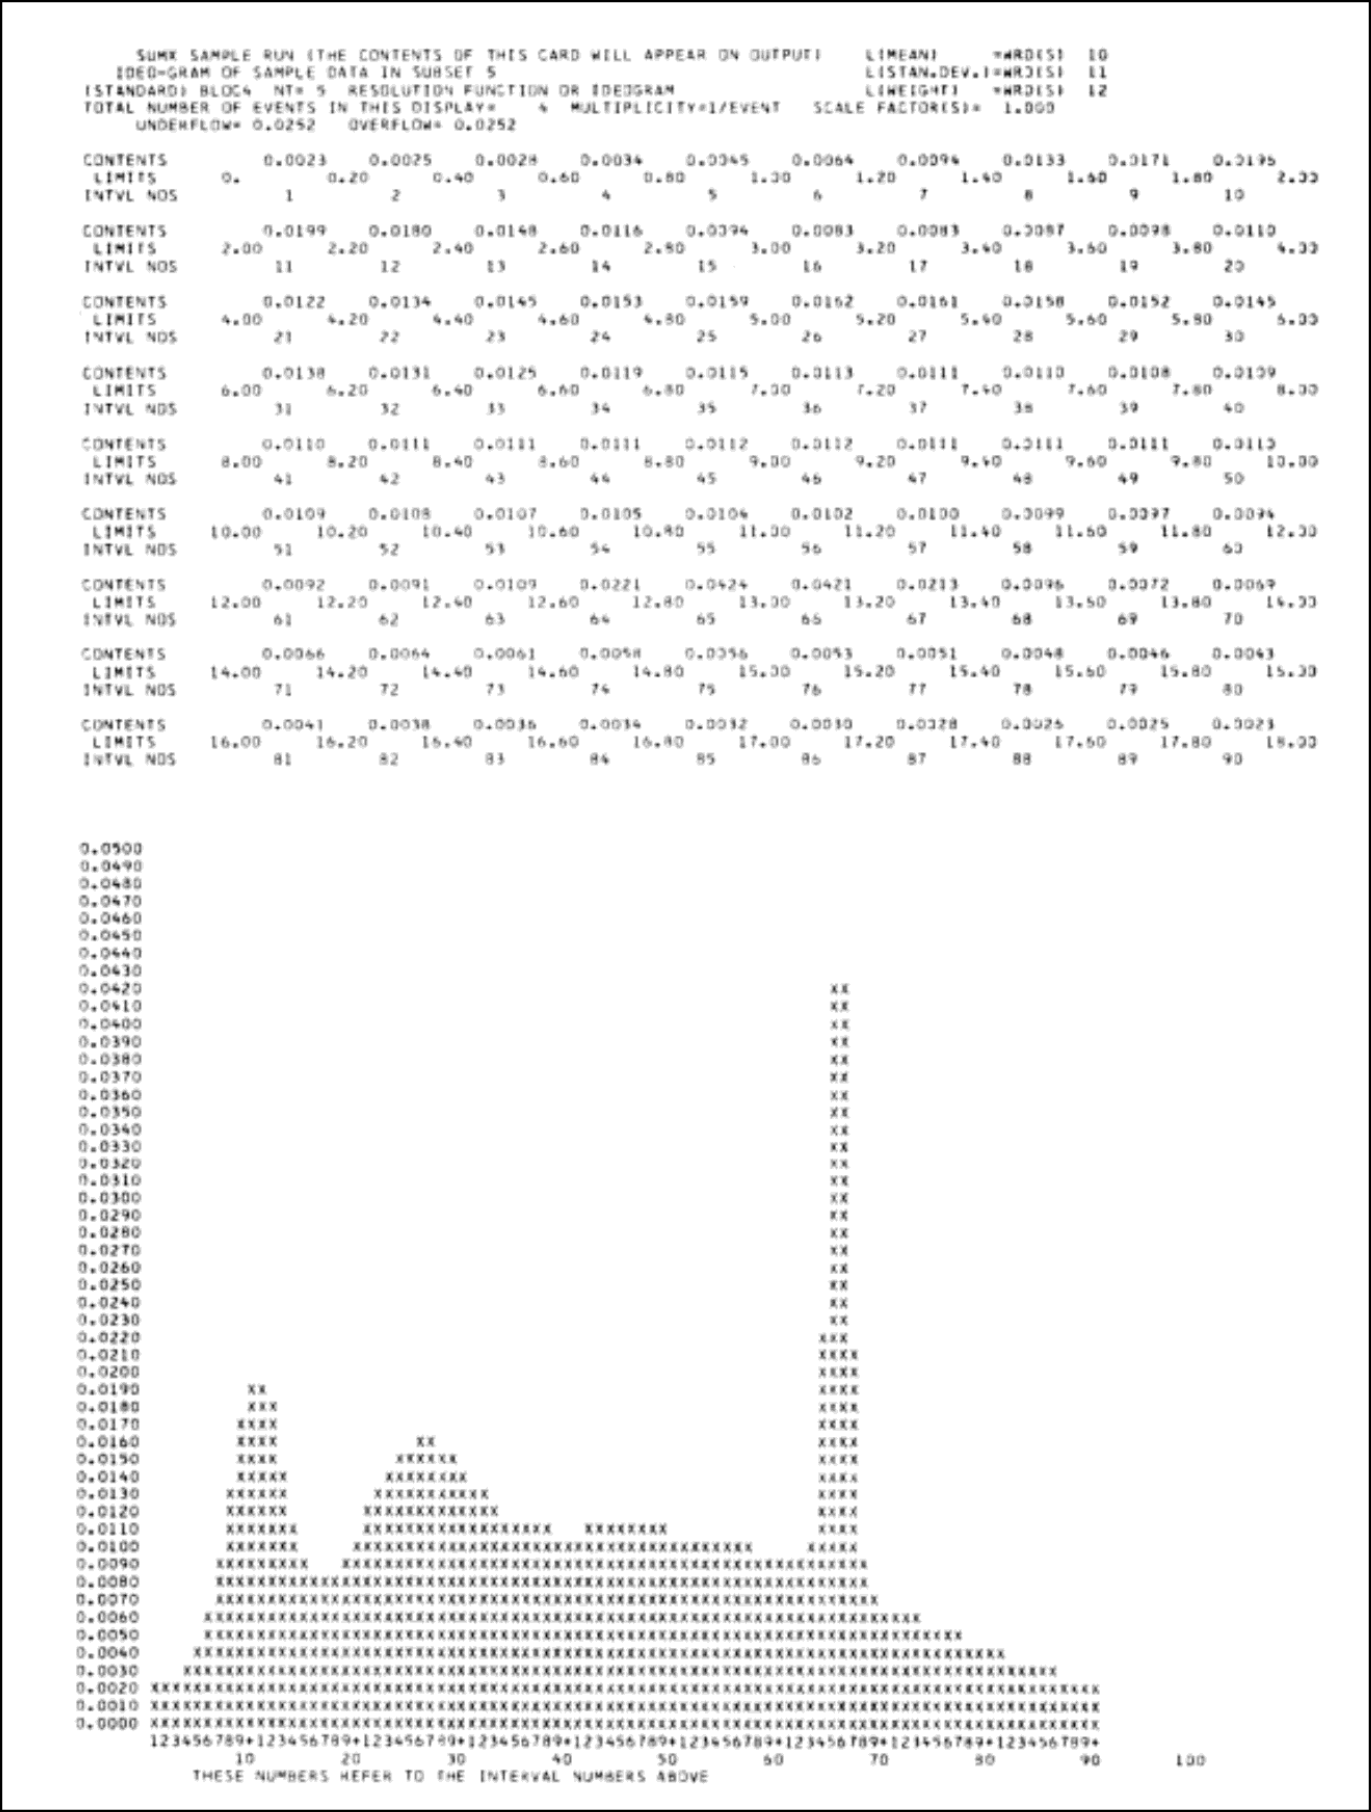
\includegraphics[height=6.5 cm]{PLOTS/sumx-histogram.png}
%% \end{columns}
%% \end{frame}

%% \begin{frame}{CERN Courier special issues on computing}
%% \large
%% \begin{columns}
%% \column{0.3\linewidth}
%% \begin{center}
%% September 1967

%% \vspace{0.2 cm}
%% 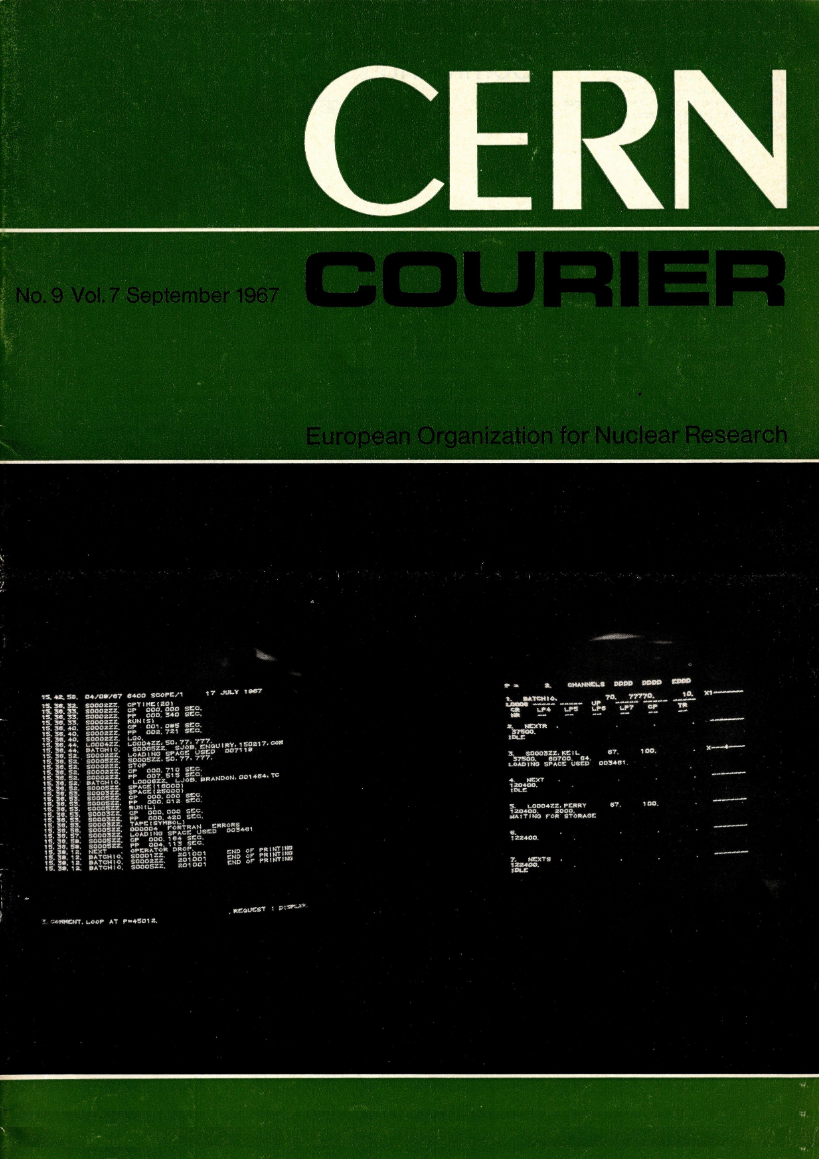
\includegraphics[width=\linewidth]{PLOTS/cern-courier-1.png}

%% \vspace{0.5 cm}
%% \end{center}

%% \column{0.13\linewidth}
%% Fortran mentioned 3 times

%% \column{0.3\linewidth}
%% \begin{center}
%% March 1972

%% \vspace{0.2 cm}
%% 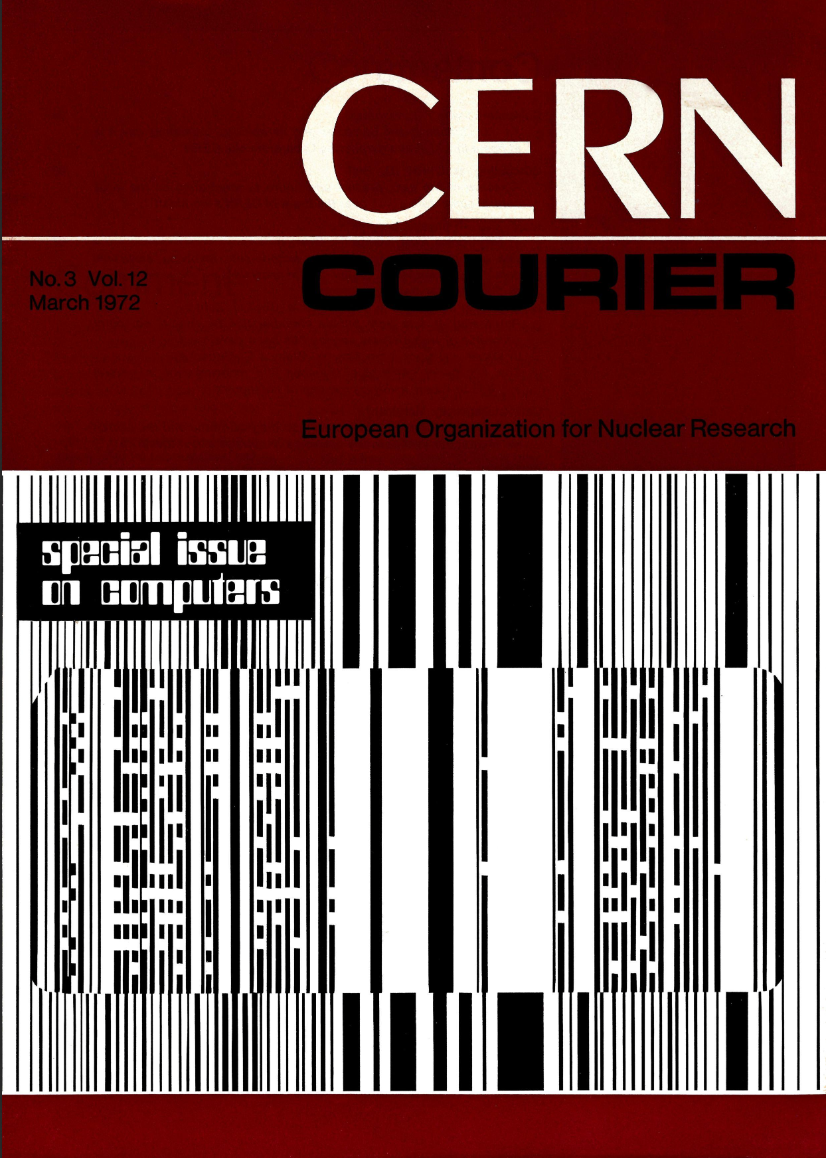
\includegraphics[width=\linewidth]{PLOTS/cern-courier-2.png}

%% \vspace{0.5 cm}
%% \end{center}

%% \column{0.13\linewidth}
%% Fortran mentioned 18 times
%% \end{columns}

%% \begin{onlyenv}<1>
%% \vspace{3 cm}
%% \end{onlyenv}\begin{onlyenv}<2>
%% \vspace{-5.8 cm}
%% \begin{columns}
%% \column{0.4\linewidth}
%% 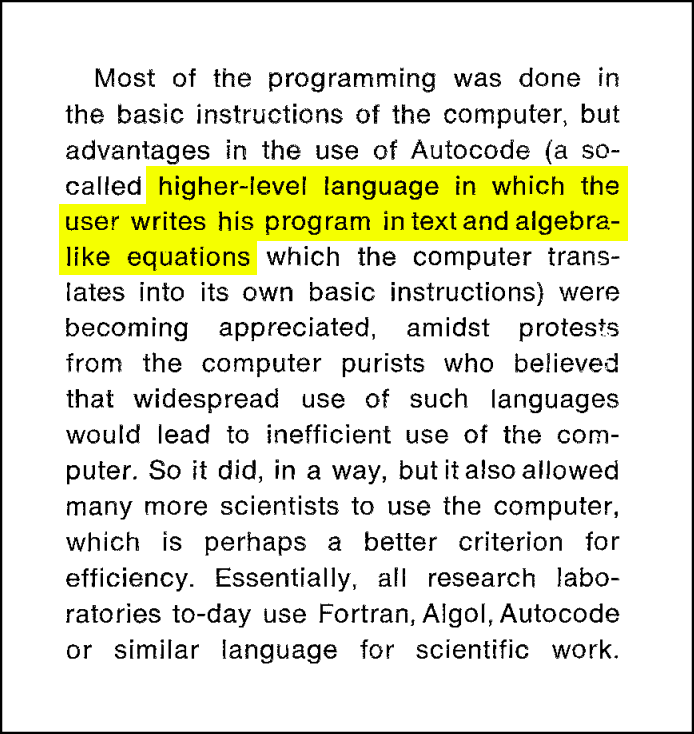
\includegraphics[width=\linewidth]{PLOTS/cern-courier-fortran-1.png}

%% \column{0.35\linewidth}
%% 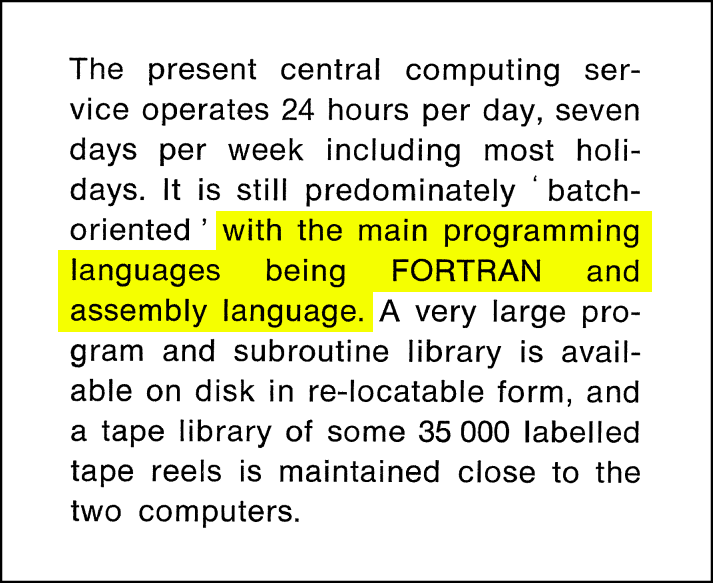
\includegraphics[width=\linewidth]{PLOTS/cern-courier-fortran-2.png}

%% \end{columns}
%% \end{onlyenv}
%% \end{frame}

%% \begin{frame}{Part 1 conclusions: adoption of Fortran}
%% \large
%% \vspace{0.5 cm}
%% NHEP adopted Fortran for data analysis in the first years after its release in 1956.

%% \vspace{0.75 cm}
%% \uncover<2->{``Algebra-like equations'' (i.e.\ {\bf FOR}mula-{\bf TRAN}slation) was an obvious benefit.}

%% \vspace{0.75 cm}
%% \uncover<3->{Also portability: assembly programs only work on a single model of computer.}

%% \vspace{0.75 cm}
%% \uncover<4->{Why Fortran and not something else (e.g.\ ALGOL)?

%% \vspace{0.1 cm}
%% \hfill It was IBM's product, and most labs were buying IBM computers.}
%% \end{frame}

%% \begin{frame}{\mbox{ }}
%% \LARGE
%% \begin{center}
%% \textcolor{darkblue}{Part 2: C++}
%% \end{center}
%% \end{frame}

%% \begin{frame}{Fortran lacked an essential feature for NHEP}
%% \scriptsize
%% \vspace{0.25 cm}
%% \begin{center}
%% 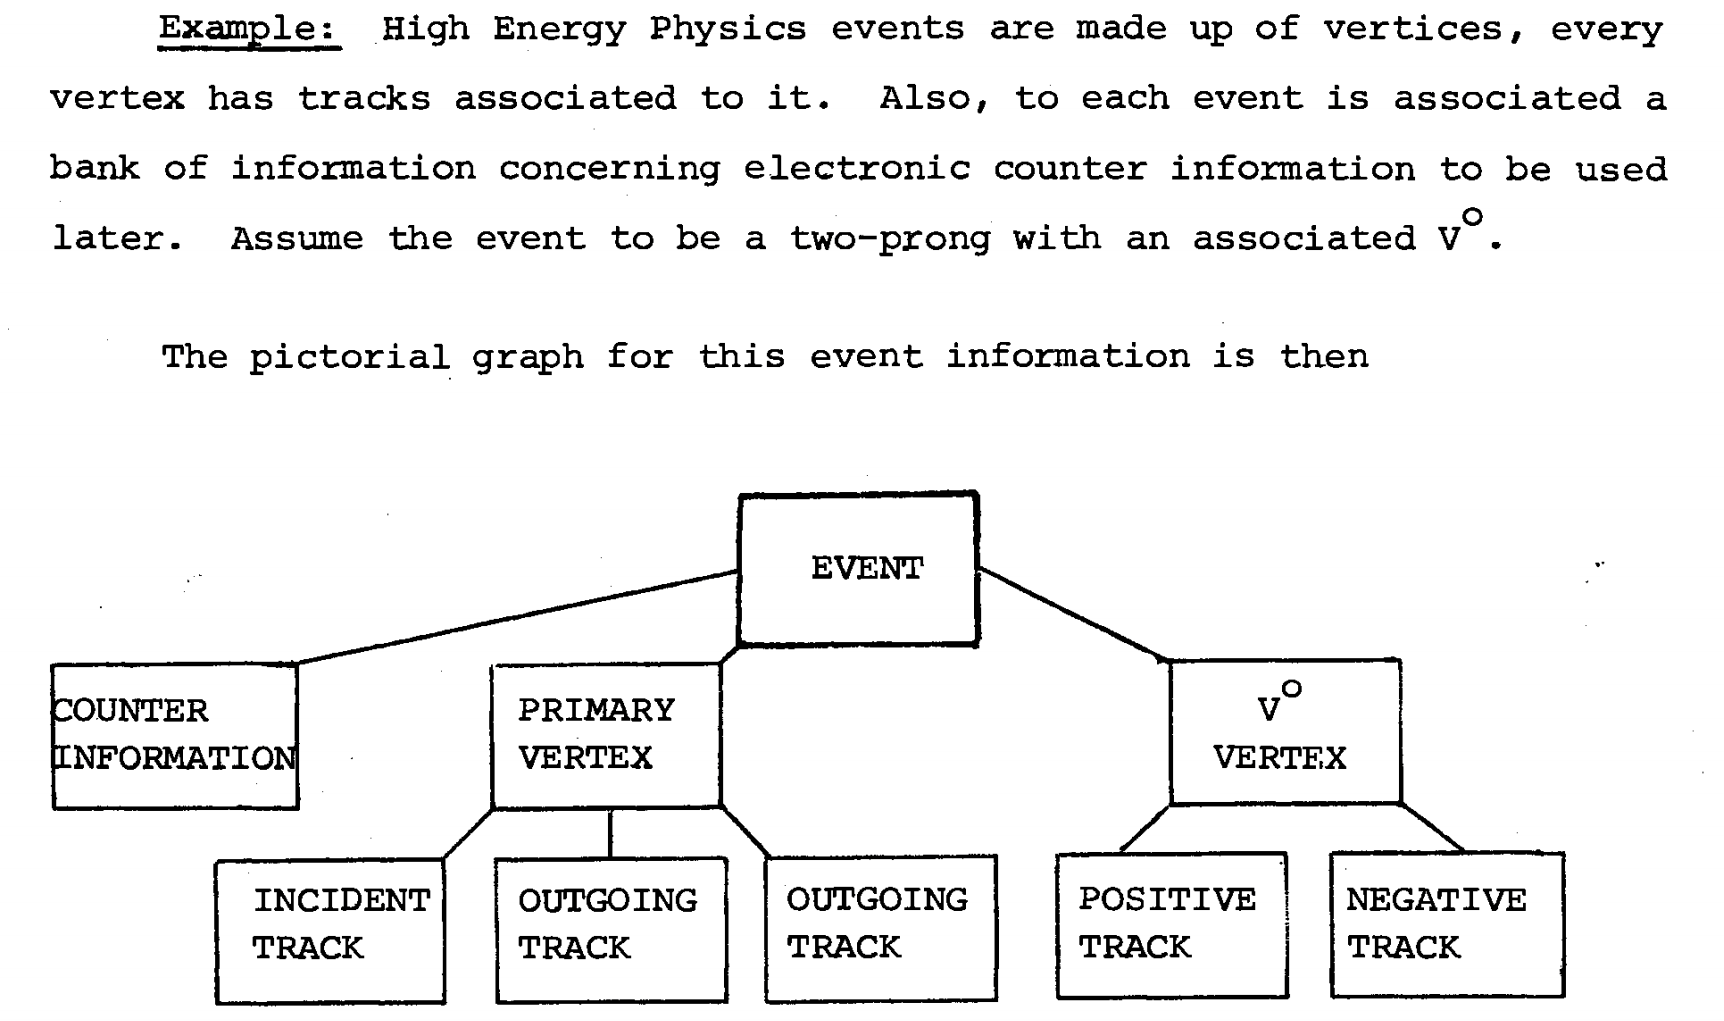
\includegraphics[width=0.87\linewidth]{PLOTS/hydra-2.png}
%% \end{center}

%% \vspace{-2 cm}
%% \hfill R.K.\ B\"ock, {\it Initiation}\hspace{-0.5 cm}

%% \hfill {\it to Hydra} (1974)\hspace{-0.5 cm}
%% \vspace{2 cm}

%% \begin{center}
%% \vspace{-6.25 cm}
%% \uncover<2->{\mbox{ }\hfill\fcolorbox{black}{white}{\begin{minipage}{0.75\linewidth}\vspace{0.75 cm}\begin{center}\begin{minipage}{0.85\linewidth}\Large This wasn't a part of Fortran until 1991. Physicists created {\it libraries} for tree-like data.\end{minipage}\end{center}\vspace{0.5 cm}\end{minipage}}\hfill\mbox{ }}
%% \vspace{6.25 cm}
%% \end{center}
%% \end{frame}

%% \begin{frame}{Fortran lacked an essential feature for NHEP}
%% \vspace{0.25 cm}
%% \begin{center}
%% \begin{minipage}{0.8\linewidth}
%% \begin{center}
%% P.\ Lebrun and A.\ Kreymer, {\it High Level Language Memory Management on Parallel Architectures} (1989)
%% \end{center}
%% \end{minipage}

%% 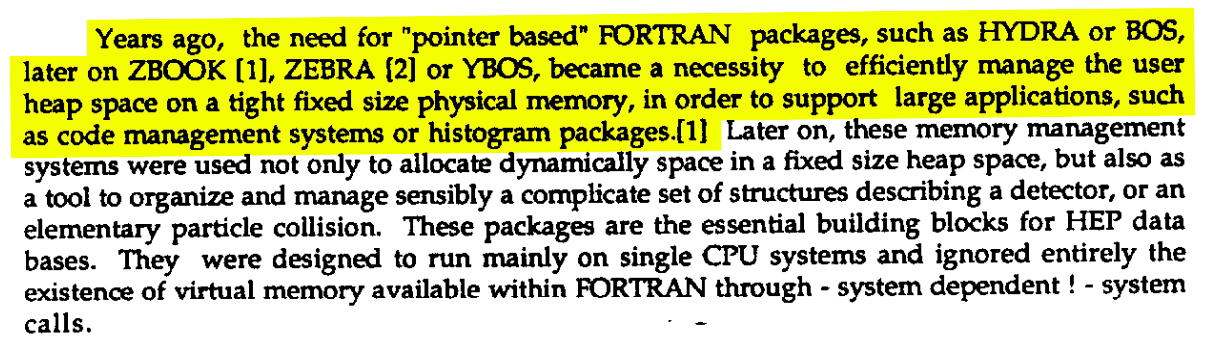
\includegraphics[width=0.9\linewidth]{PLOTS/lebrun-kreymer-zebra.png}
%% \end{center}
%% \end{frame}

%% \begin{frame}{Fortran lacked an essential feature for NHEP}
%% \scriptsize
%% \vspace{0.25 cm}
%% \begin{center}
%% 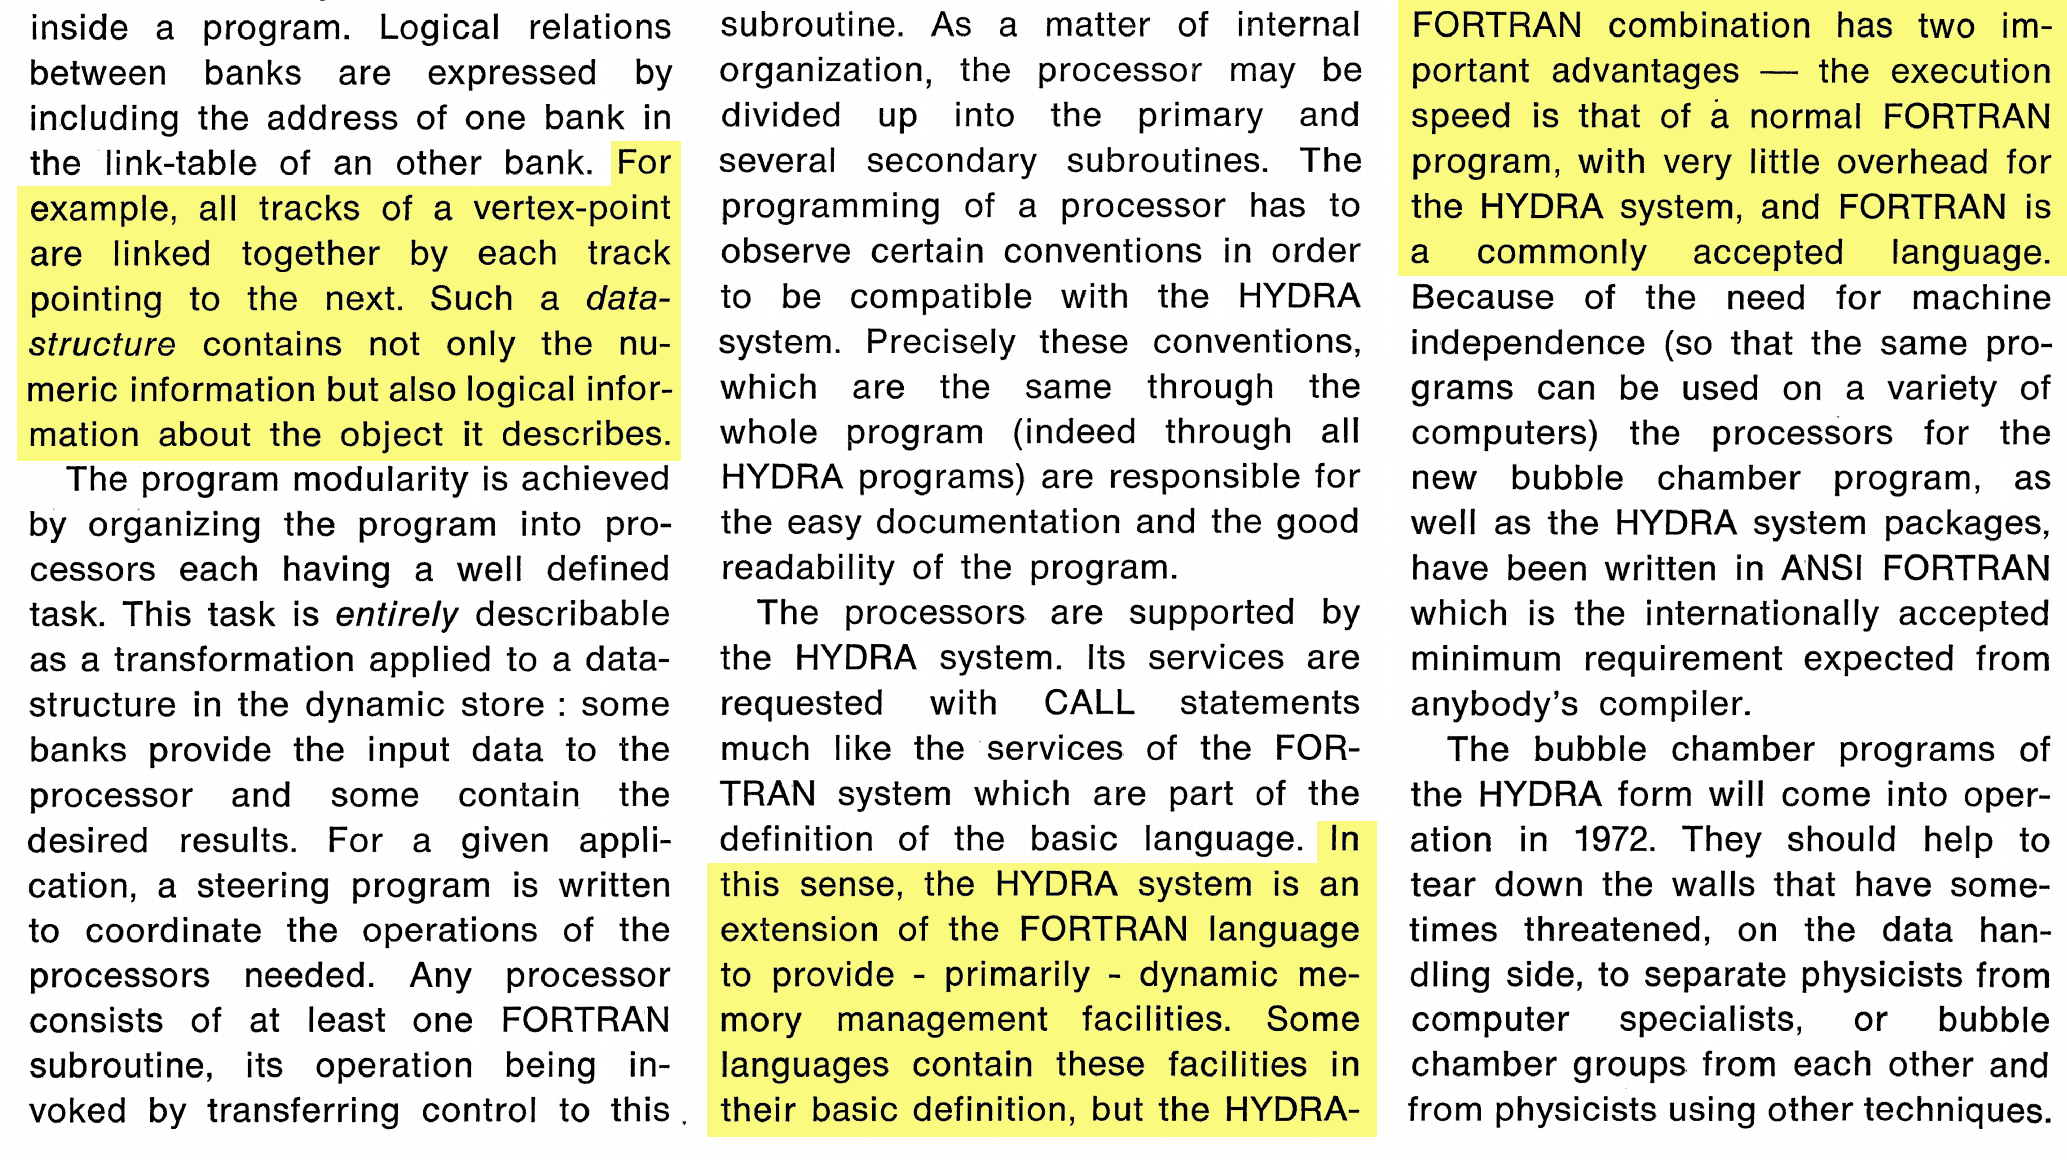
\includegraphics[width=0.85\linewidth]{PLOTS/hydra-1.png}

%% R.K.\ B\"ock and J.\ Zoll, {\it Central Computers in the Analysis}, CERN Courier No.\ 3, Vol.\ 12, March 1972
%% \end{center}
%% \end{frame}

%% \begin{frame}[fragile]{Beyond Fortran, data structures were a common language feature}
%% \small
%% \vspace{0.5 cm}
%% \begin{columns}[t]
%% \column{0.31\linewidth}
%% {\large COBOL (1959)}

%% \begin{verbatim}
%% 01 Point.
%%    05 x    pic 9(3).
%%    05 y    pic 9(3).
%% \end{verbatim}

%% \column{0.31\linewidth}
%% {\large Simula (1962)}

%% \begin{verbatim}
%% Class Point (x, y);
%%   Integer x, y;
%%   ! define attributes...
%%   ! define methods...
%% End of Point;
%% \end{verbatim}

%% \column{0.31\linewidth}
%% {\large PL/I (1964)}

%% \begin{verbatim}
%% define structure
%%   1 point,
%%      2 x integer,
%%      2 y integer;
%% \end{verbatim}

%% \end{columns}

%% \vspace{1 cm}
%% \begin{columns}[t]
%% \column{0.31\linewidth}
%% {\large ALGOL-68 (1968)}

%% \begin{verbatim}
%% MODE POINT = STRUCT(
%%    INT x,
%%    INT y
%% );
%% \end{verbatim}

%% \column{0.31\linewidth}
%% {\large Pascal (1970)}

%% \begin{minted}{pascal}
%% type Point = record
%%     x, y: integer;
%% end;
%% \end{minted}

%% \column{0.31\linewidth}
%% {\large C (1972)}

%% \begin{minted}{c}
%% typedef struct Point {
%%   int x;
%%   int y;
%% } Point;
%% \end{minted}

%% \end{columns}
%% \end{frame}

%% \begin{frame}{Beyond Fortran, data structures were a common language feature}
%% \vspace{0.5 cm}
%% \begin{center}
%% \begin{minipage}{0.8\linewidth}
%% \begin{center}
%% Paul Kunz, {\it Physics Analysis Tools} (1991)
%% \end{center}
%% \end{minipage}

%% \vspace{0.25 cm}
%% 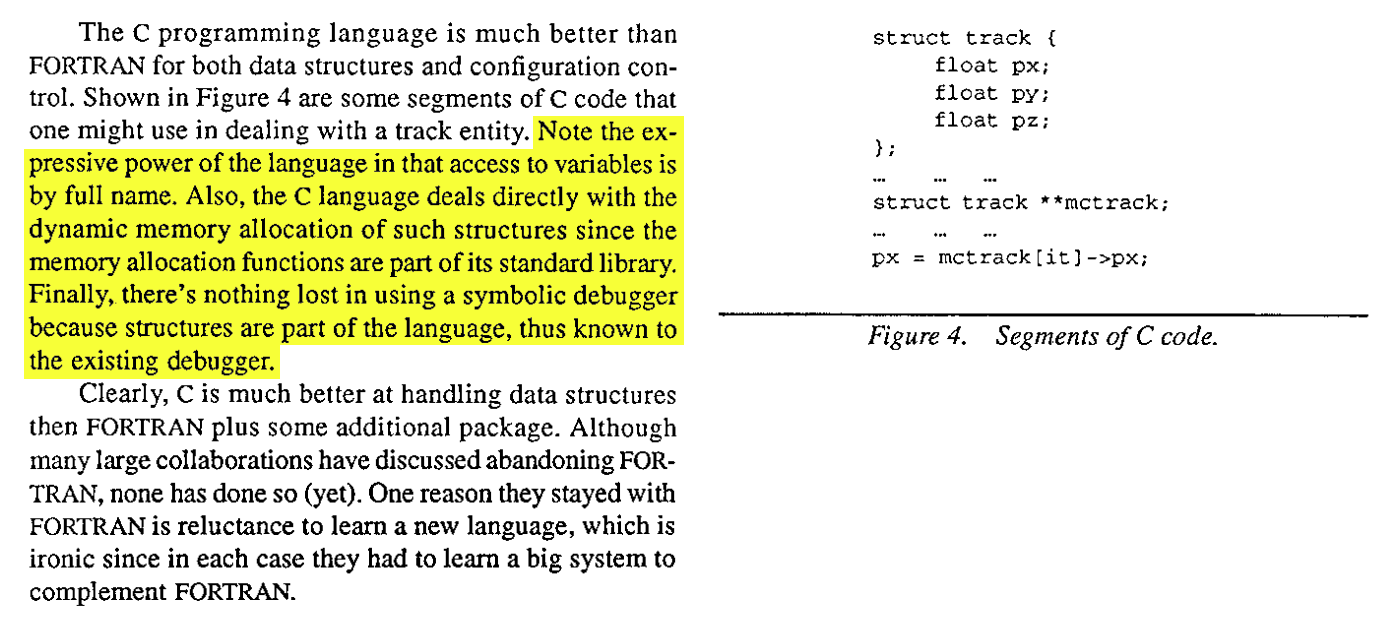
\includegraphics[width=0.9\linewidth]{PLOTS/kunz-physics-analysis-tools.png}
%% \end{center}

%% \begin{uncoverenv}<2->
%% \vspace{-2.25 cm}
%% \hfill\begin{minipage}{0.48\linewidth}
%% In the first 15 years of CHEP (1985--2000), similar suggestions were made for ALGOL, PL/I, Pascal, Ada, Eiffel, Objective C, Java, and of course C++.
%% \end{minipage}\hspace{-0.25 cm}
%% \vspace{1.5 cm}
%% \end{uncoverenv}
%% \end{frame}

%% \begin{frame}[fragile]{Fortran did finally add data structures}
%% \vspace{0.25 cm}
%% \begin{columns}
%% \column{0.3\linewidth}
%% {\large Fortran-90 (1991)}
%% \small
%% \begin{minted}{fortran}
%% type Point
%%     integer :: x
%%     integer :: y
%% end type Point
%% \end{minted}
%% \vspace{2 cm}

%% \column{0.58\linewidth}
%% \begin{uncoverenv}<2->

%% Ren\'e Brun, {\it Technologies, Collaborations and Languages: 20 Years of HEP Computing} (2012)

%% \vspace{0.25 cm}
%% 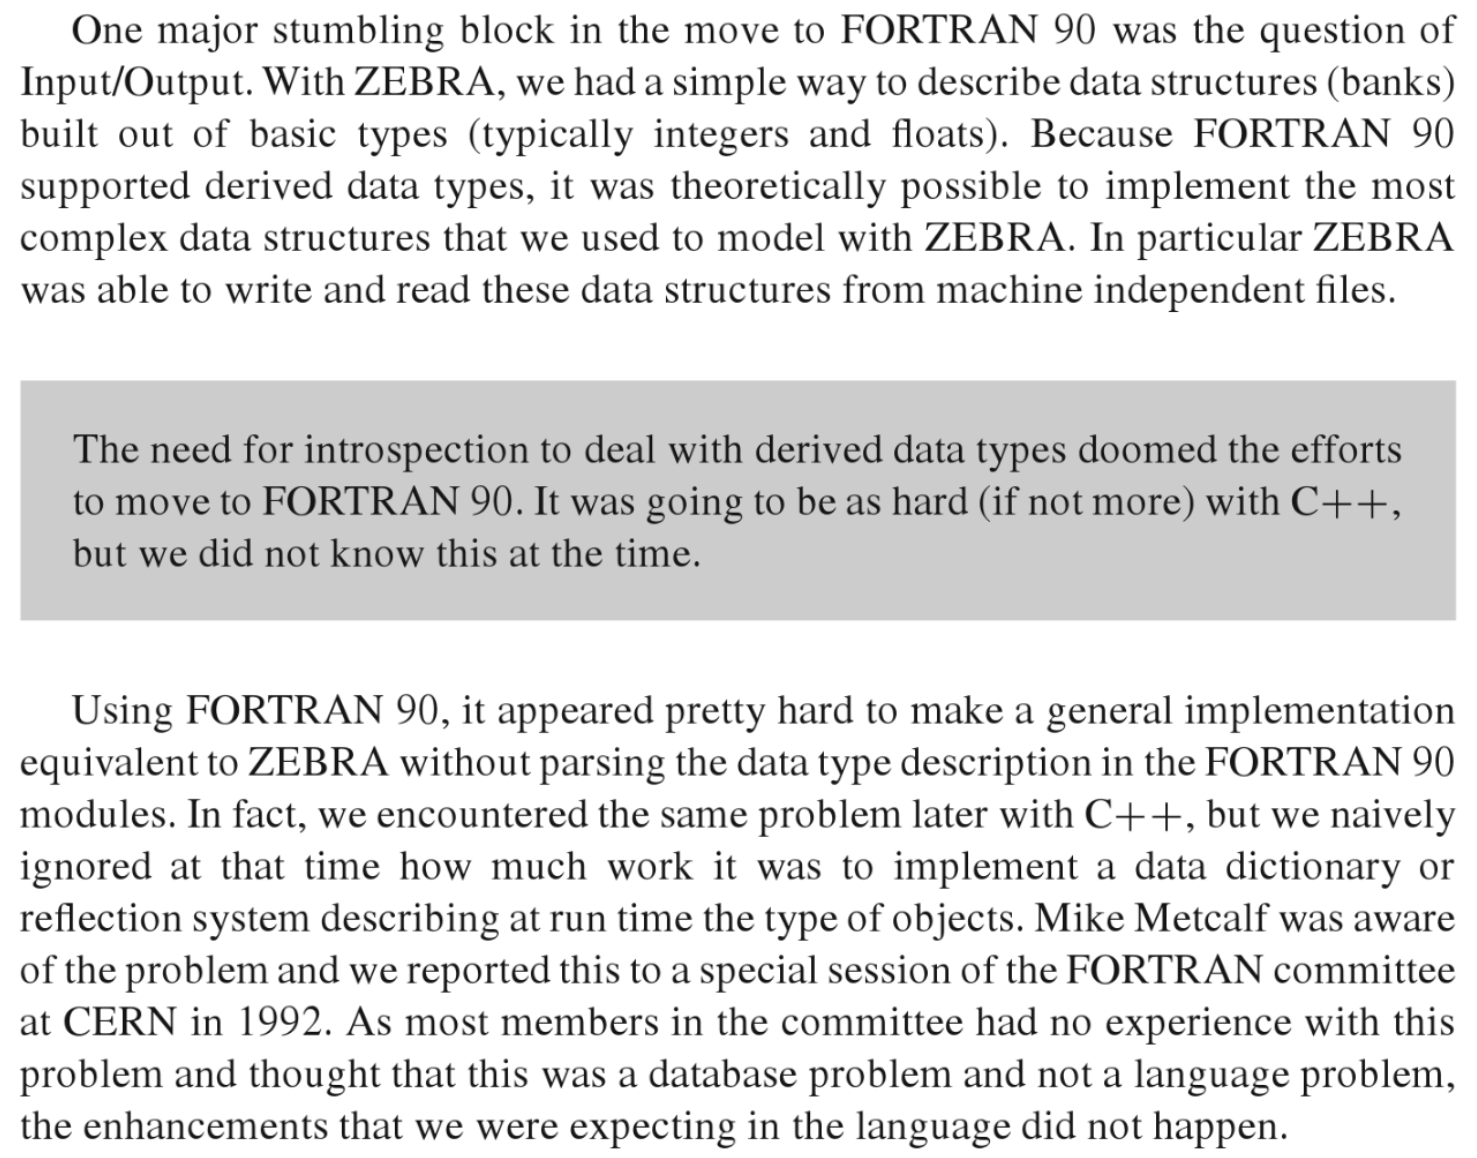
\includegraphics[width=\linewidth]{PLOTS/brun-20-years-of-hep-computing.png}
%% \end{uncoverenv}
%% \end{columns}
%% \end{frame}

%% \begin{frame}{\mbox{ }}
%% \Large
%% \vspace{0.25 cm}
%% So actually, NHEP needs:

%% \vspace{0.25 cm}
%% \begin{enumerate}\setlength{\itemsep}{0.15 cm}
%% \item rich data structures in the programming language,
%% \item serialization of those structures to/from disk,
%% \item read compatibility for old data versions (schema evolution),
%% \item mapping between persistent data and language's structures (which can be implemented with type-introspection).
%% \end{enumerate}

%% \large
%% \vspace{0.5 cm}
%% \uncover<2->{HYDRA/ZEBRA/etc.\ approached these as one problem.}

%% \vspace{0.25 cm}
%% \uncover<3->{In Java, \textcolor{darkblue}{(1--2)} is a language problem, \textcolor{darkblue}{(3--4)} is for databases.}

%% \vspace{0.25 cm}
%% \uncover<4->{Object databases focus on \textcolor{darkblue}{(4)} as the real problem\ldots}
%% \end{frame}

%% \begin{frame}{\mbox{ }}
%% \vspace{0.35 cm}
%% \Large
%% \begin{center}
%% So it wasn't just a matter of adding another language to the mix.

%% \vspace{1 cm}
%% The whole infrastructure had to change.

%% \vspace{1 cm}
%% \textcolor{darkblue}{You only want to do that once!}
%% \end{center}
%% \end{frame}

%% \begin{frame}{Programming languages in CHEP title/abstract regex matches}
%% \vspace{0.15 cm}
%% \begin{columns}
%% \column{1.1\linewidth}
%% 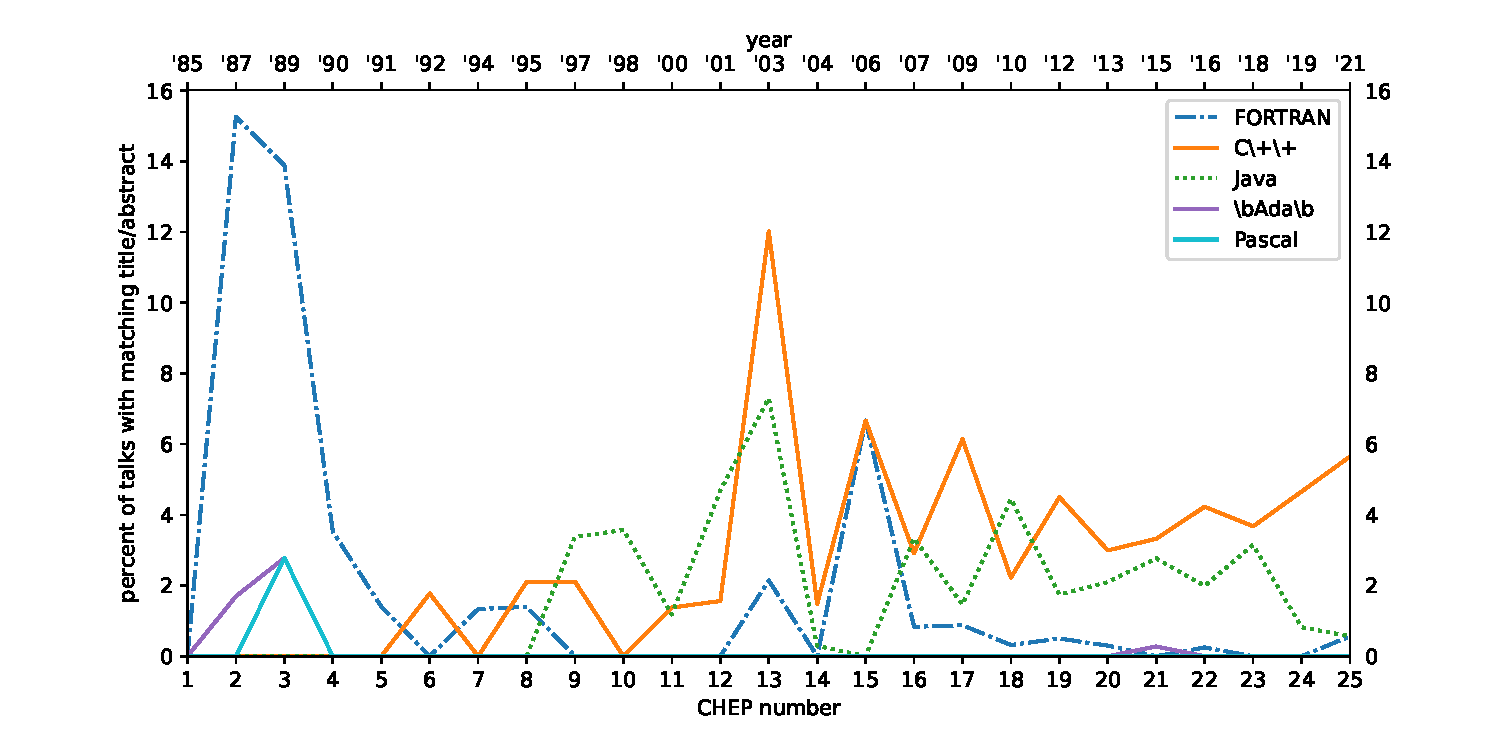
\includegraphics[width=\linewidth]{PLOTS/chep-papers-language-1.pdf}
%% \end{columns}
%% \end{frame}

%% \begin{frame}{Data infrastructure in CHEP title/abstract regex matches}
%% \vspace{0.15 cm}
%% \begin{columns}
%% \column{1.1\linewidth}
%% 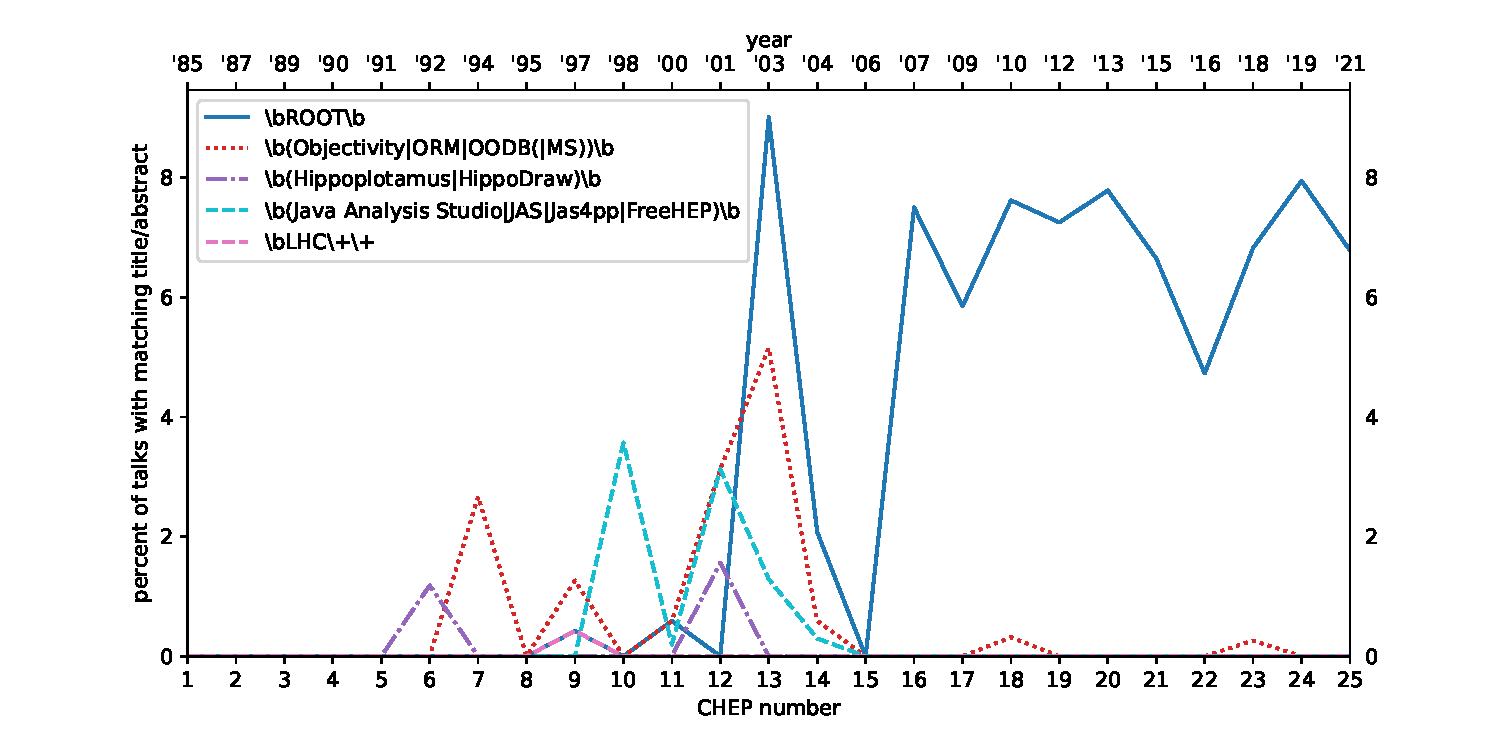
\includegraphics[width=\linewidth]{PLOTS/chep-papers-package-1.pdf}
%% \end{columns}
%% \end{frame}

%% \begin{frame}{Total number of talks (denominator): dips are small CHEPs}
%% \vspace{0.15 cm}
%% \begin{columns}
%% \column{1.1\linewidth}
%% 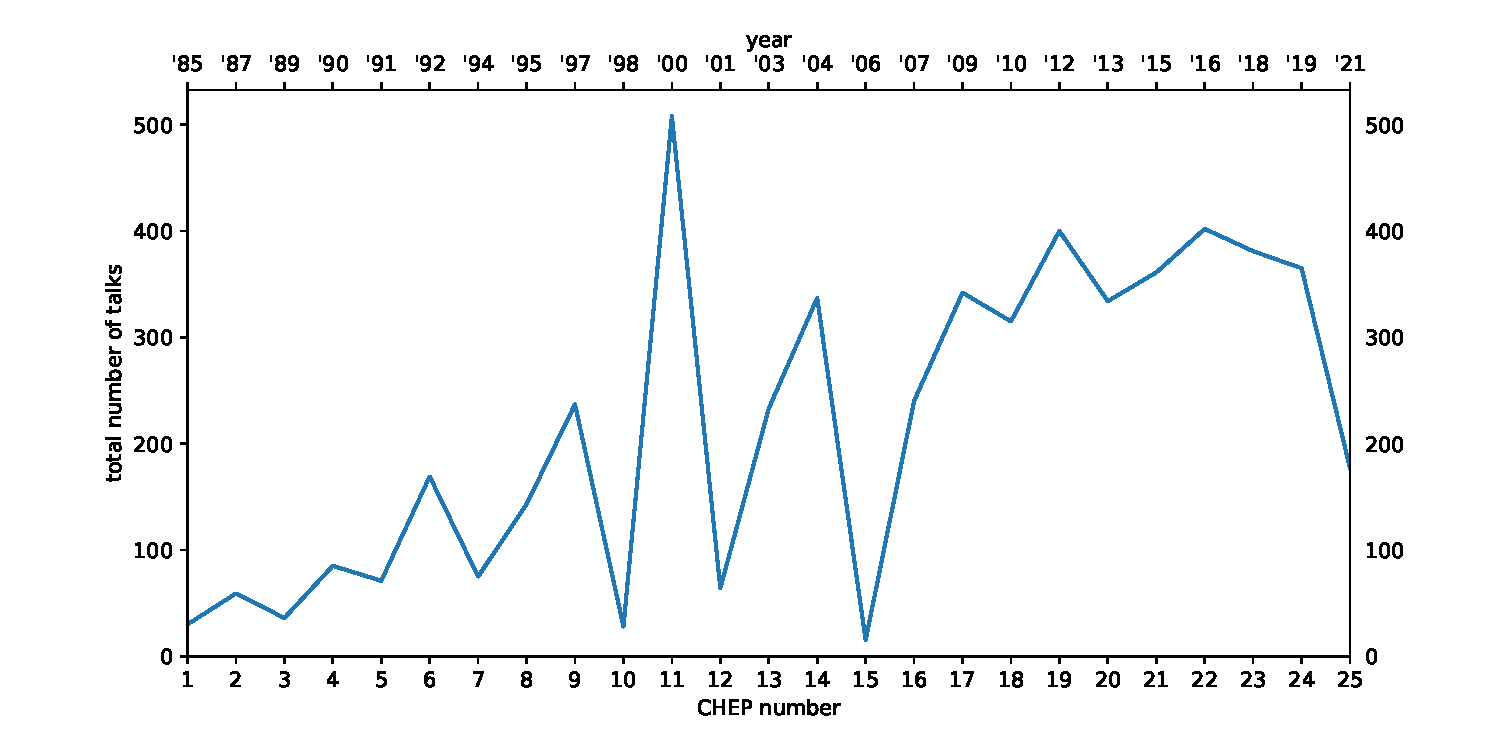
\includegraphics[width=\linewidth]{PLOTS/chep-papers-denominator.pdf}
%% \end{columns}
%% \end{frame}

%% \begin{frame}{ROOT I/O is custom, but was more advanced than alternatives}
%% \vspace{0.1 cm}
%% \begin{center}
%% 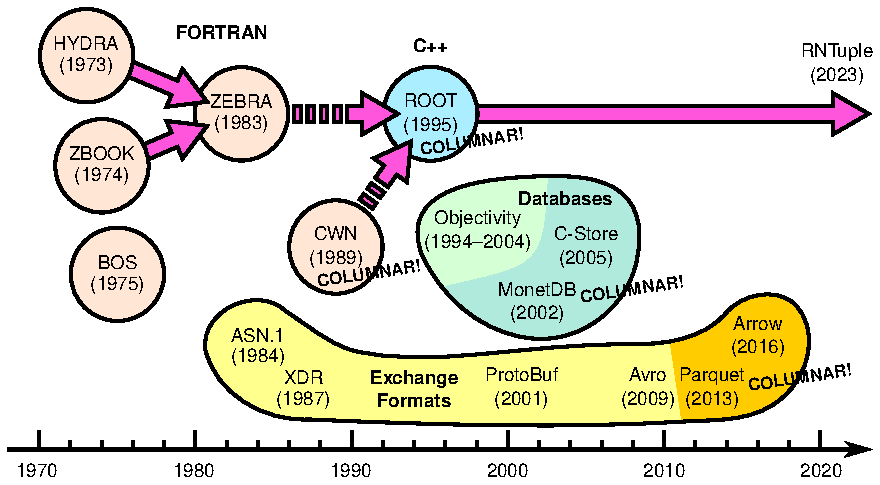
\includegraphics[width=\linewidth]{PLOTS/history.pdf}
%% \end{center}
%% \end{frame}

%% \begin{frame}{Some advances had to be rediscovered outside NHEP}
%% \large
%% \vspace{0.25 cm}
%% \begin{center}
%% {\it Dremel: Interactive Analysis of Web-Scale Datasets} (Google, 2010)

%% \vspace{0.25 cm}
%% \fbox{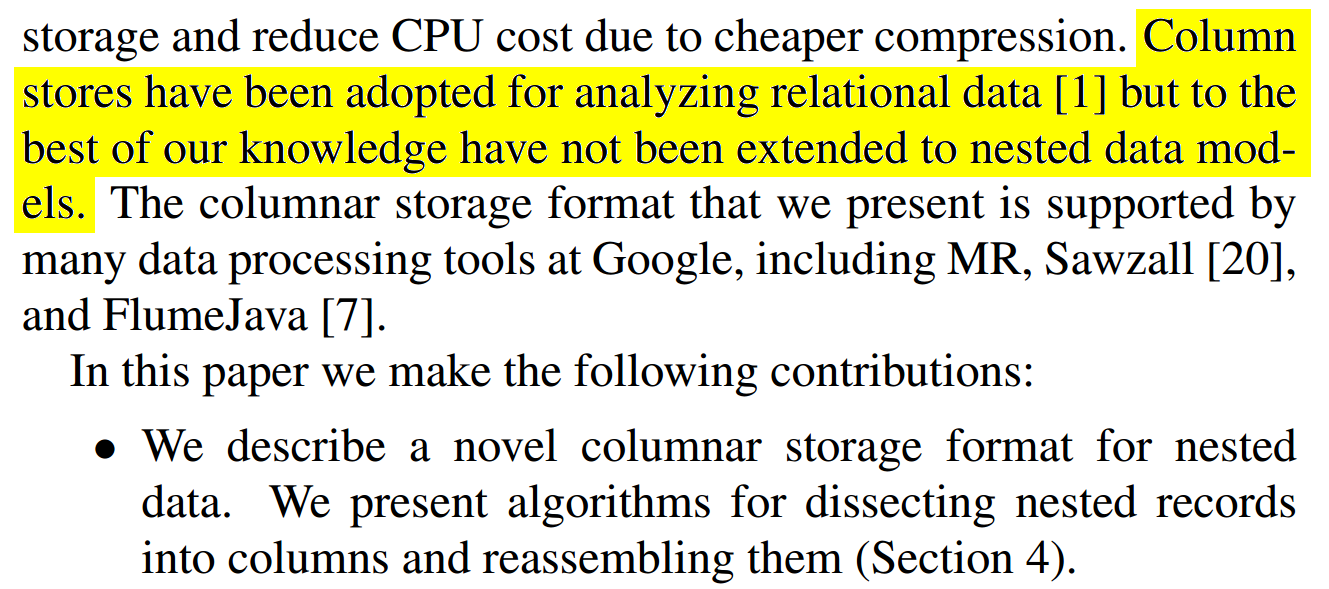
\includegraphics[width=0.7\linewidth]{PLOTS/dremel.png}}

%% \vspace{0.25 cm}
%% Columnar, nested data was a ROOT feature 15 years earlier.
%% \end{center}
%% \end{frame}

%% \begin{frame}{Part 2 conclusions: adoption of C++}
%% \large
%% \vspace{0.5 cm}
%% NHEP adoption of C++ (or similar) was held back by the fact that we had unique infrastructure.

%% \vspace{0.75 cm}
%% \uncover<2->{Data structures are important, but so is serialization.}

%% \vspace{0.75 cm}
%% \uncover<3->{Our solutions were both more advanced and less modular than others.}

%% \vspace{0.75 cm}
%% \uncover<4->{Many options considered in late 1990's; C++ with ROOT I/O became dominant.}
%% \end{frame}

\begin{frame}{\mbox{ }}
\LARGE
\begin{center}
\textcolor{darkblue}{Part 3: Python}
\end{center}
\end{frame}

\begin{frame}{End-stage data analysis benefits from interactivity}
\vspace{0.25 cm}
\begin{columns}
\column{0.35\linewidth}
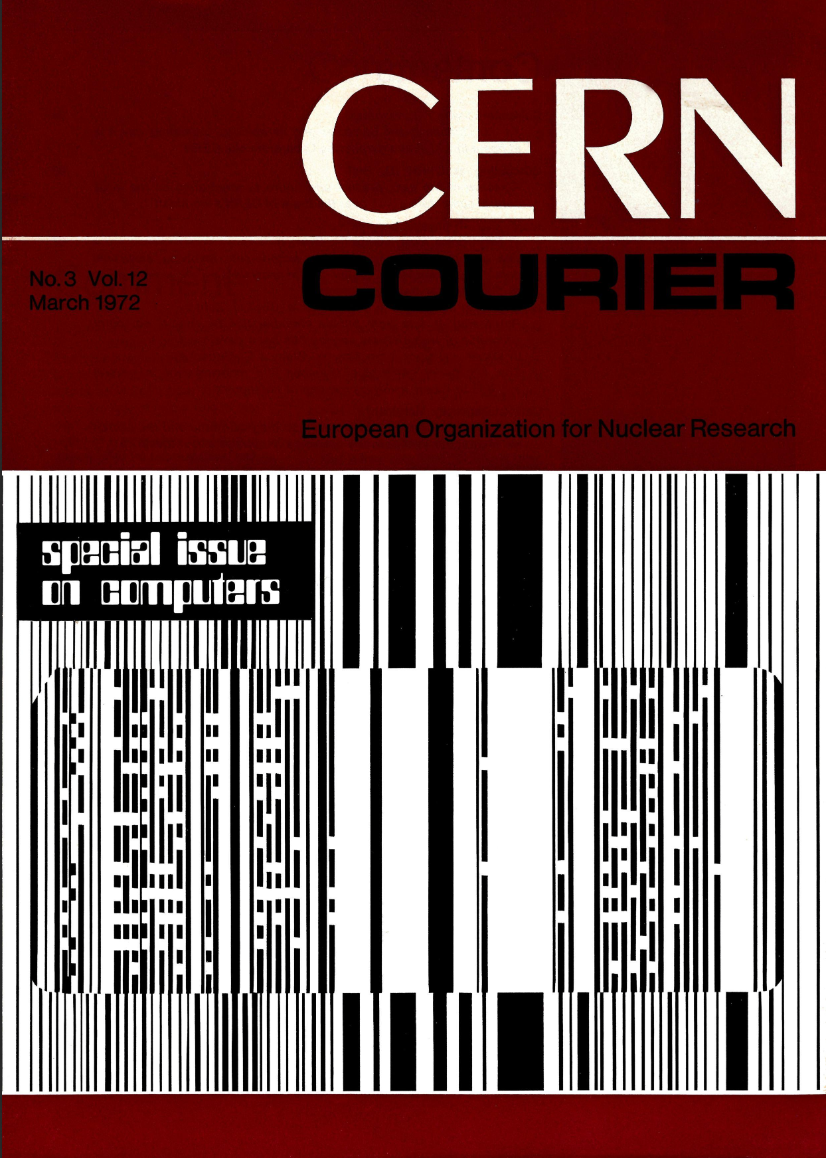
\includegraphics[width=\linewidth]{PLOTS/cern-courier-2.png}

\column{0.65\linewidth}
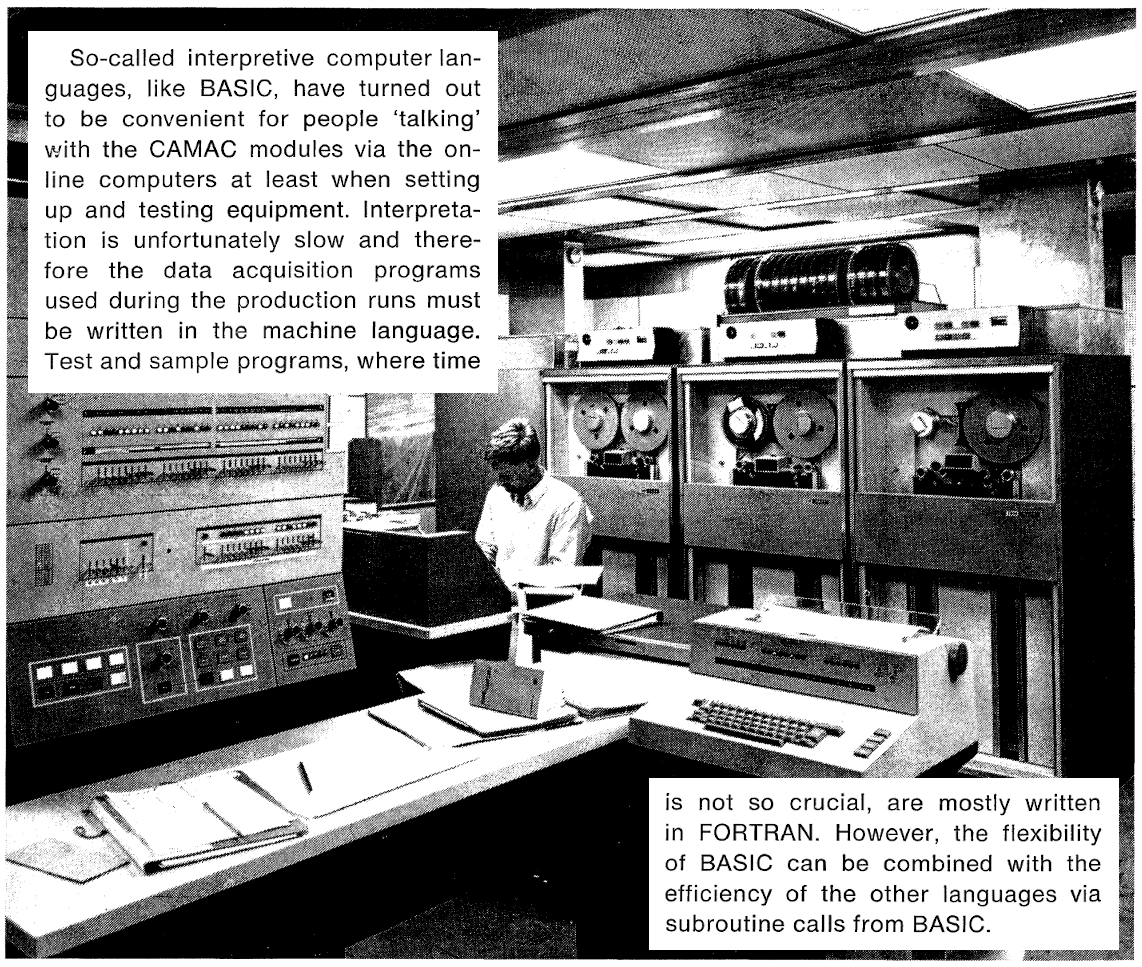
\includegraphics[width=\linewidth]{PLOTS/cern-courier-basic.png}
\end{columns}
\end{frame}

\begin{frame}{\mbox{ }}
\vspace{0.5 cm}
\Large
NHEP has a history of custom solutions for interactivity: SPEAKEASY, Minuit, PAW, KUIP, CINT, Cling\ldots

\vspace{1 cm}
But the number of industry solutions is also vast: awk, tcl, perl\ldots
\end{frame}

\begin{frame}{In recent years, the industry has consolidated on Python}
\large
\vspace{0.25 cm}
Python is currently leading every ``most popular programming language'' index.

\vspace{0.25 cm}
\begin{columns}[t]
\column{0.33\linewidth}
\centering Tiobe

\vspace{0.1 cm}
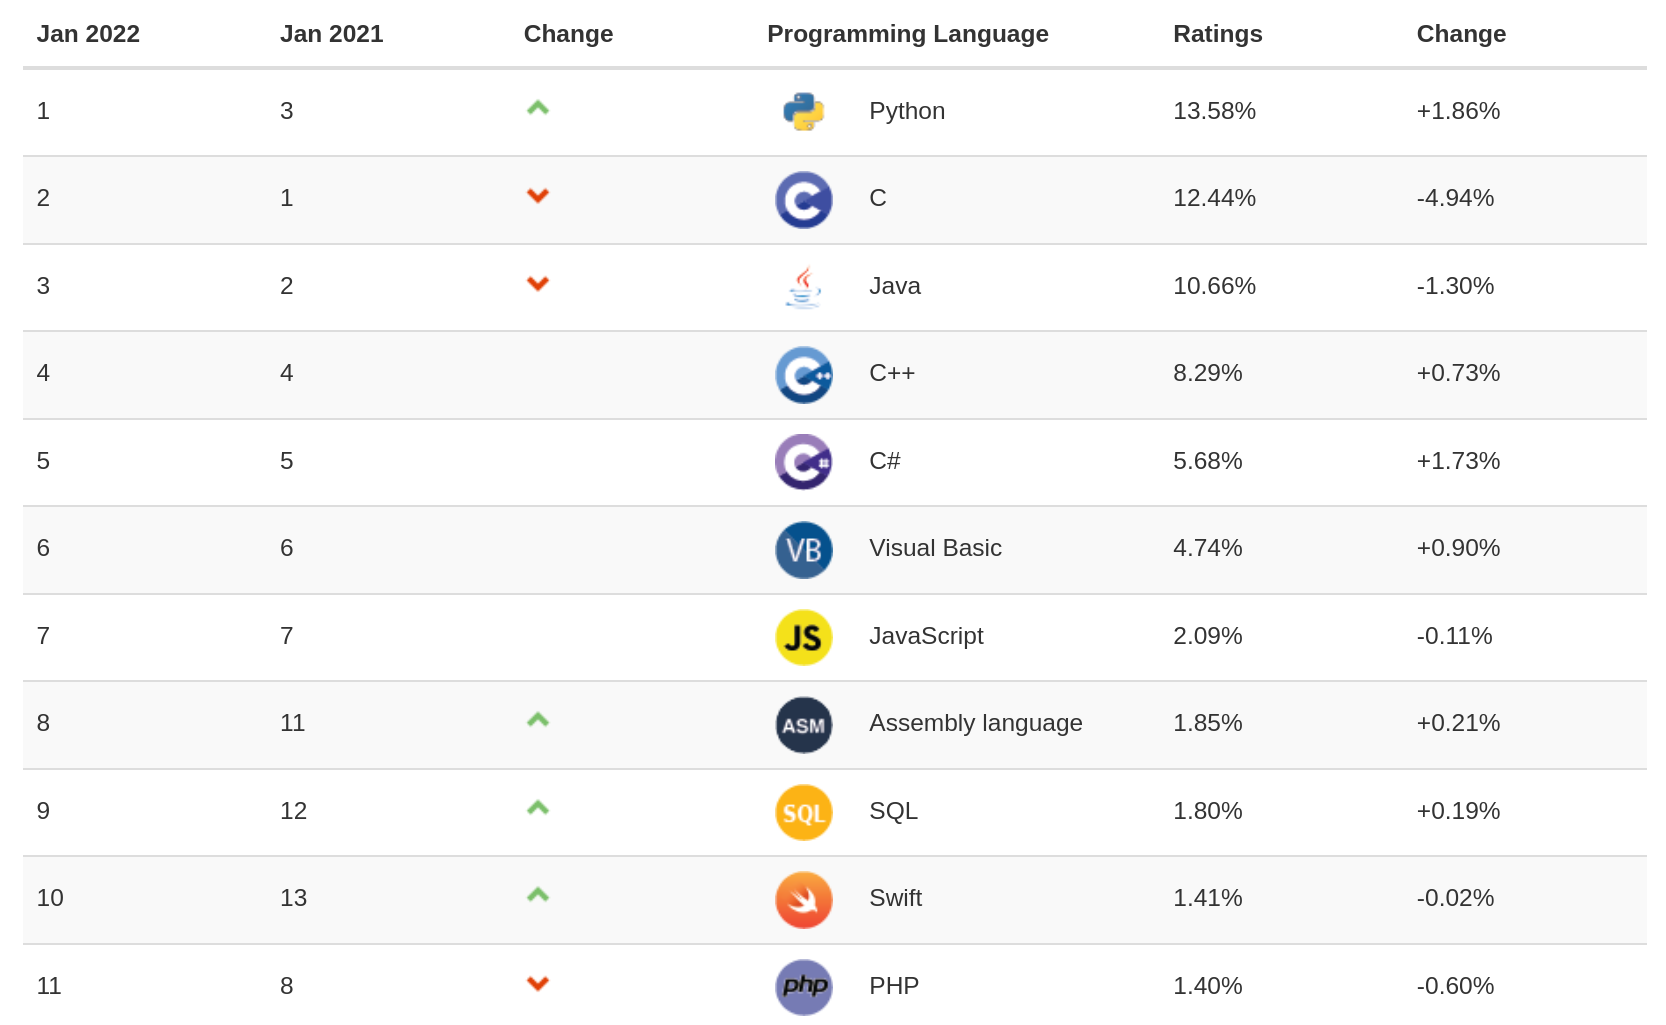
\includegraphics[width=\linewidth]{PLOTS/python-rankings-tiobe-2022.png}

\column{0.33\linewidth}
\centering PYPL

\vspace{0.1 cm}
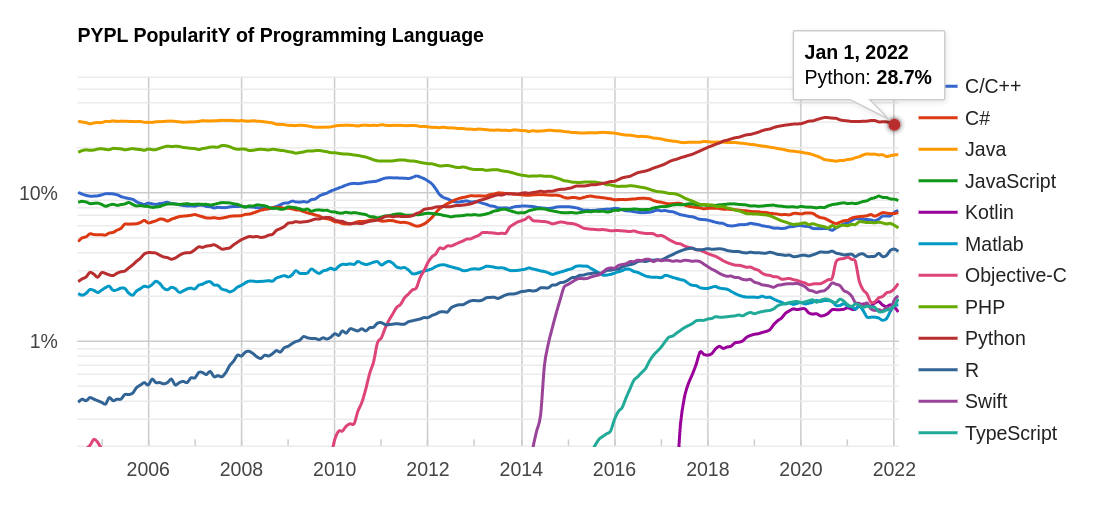
\includegraphics[width=\linewidth]{PLOTS/python-rankings-pypl-2022.png}

\column{0.33\linewidth}
\centering Google Trends

\vspace{0.1 cm}
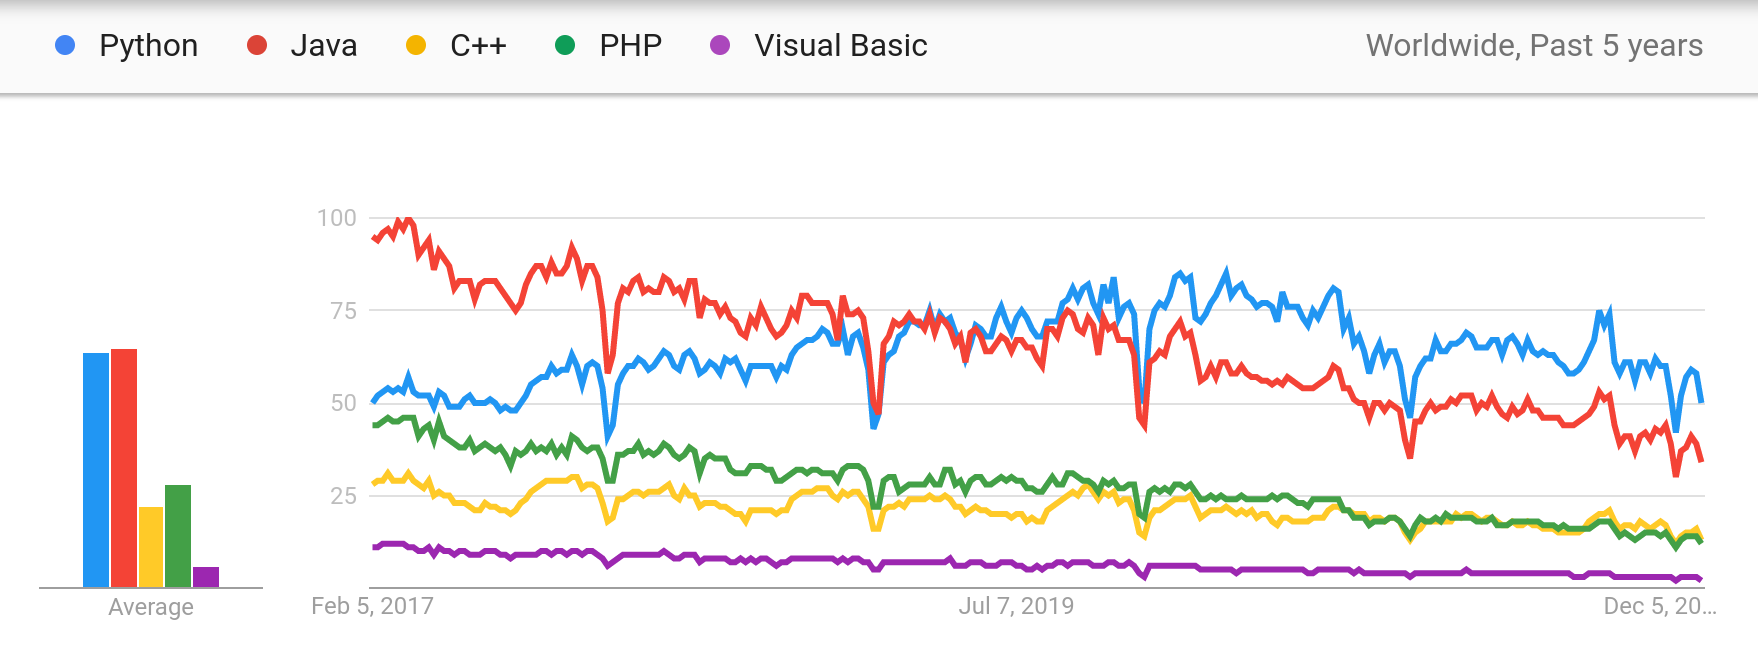
\includegraphics[width=\linewidth]{PLOTS/python-rankings-googletrends-2022.png}
\end{columns}

\vspace{0.25 cm}
\begin{columns}[t]
\column{0.5\linewidth}
\centering GitHut

\vspace{0.1 cm}
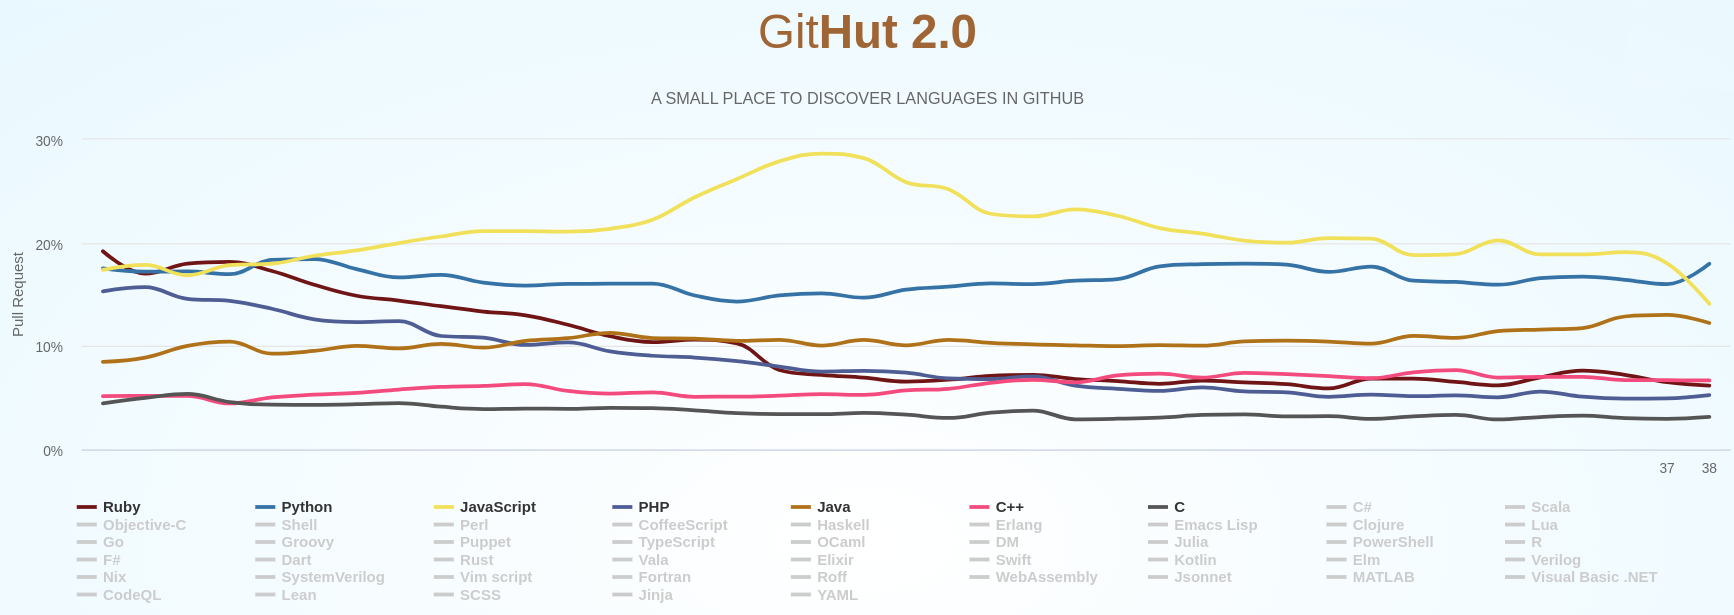
\includegraphics[width=\linewidth]{PLOTS/python-rankings-githut-2022.png}

\column{0.45\linewidth}
\centering StackOverflow

\vspace{0.1 cm}
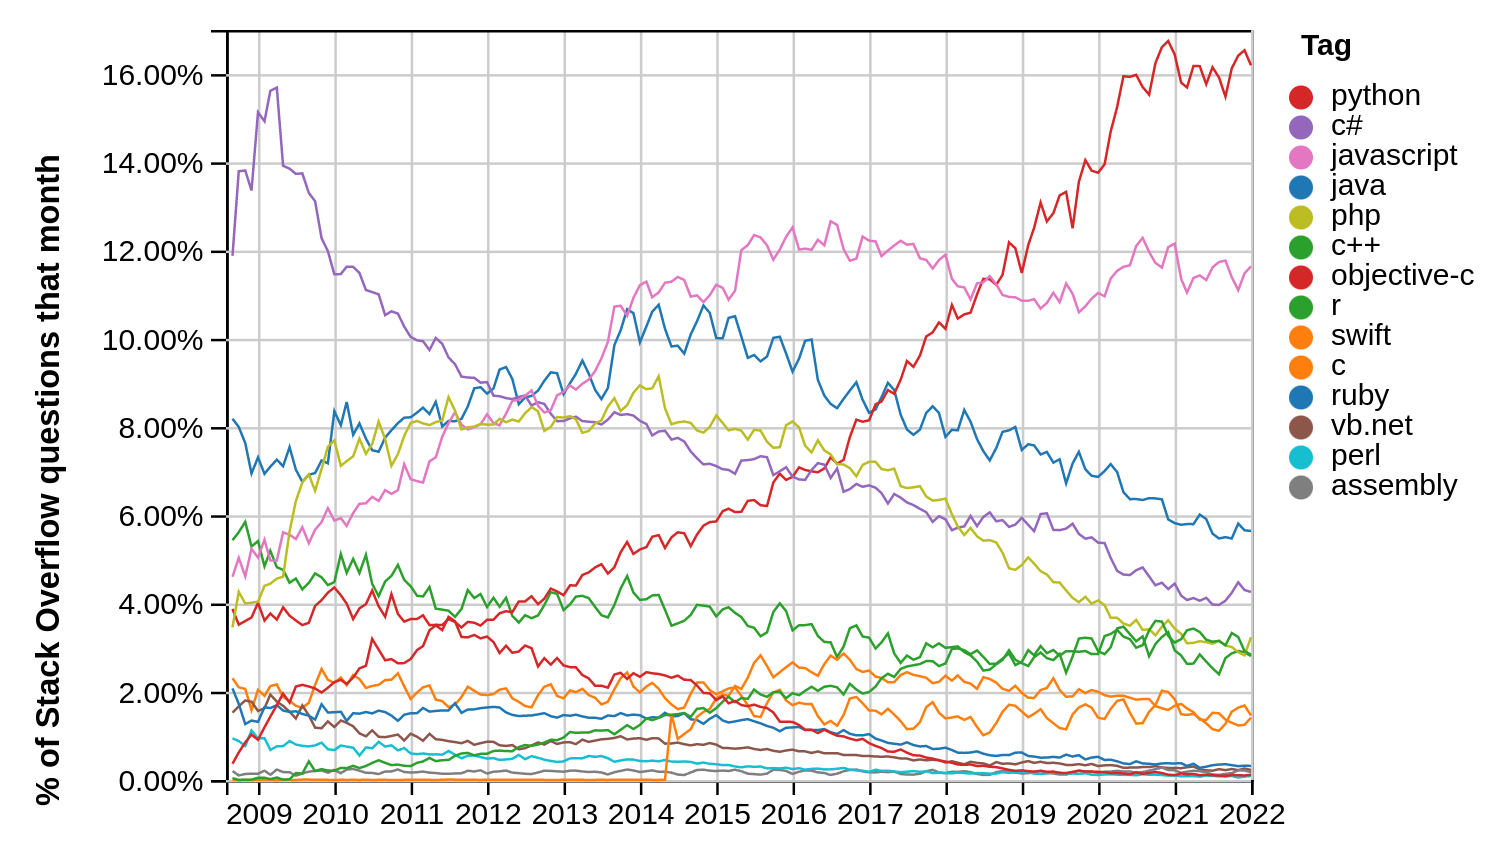
\includegraphics[width=\linewidth]{PLOTS/python-rankings-stackoverflow-2022.png}
\end{columns}
\end{frame}

\begin{frame}{Including data analytics and especially machine learning}
\vspace{0.65 cm}
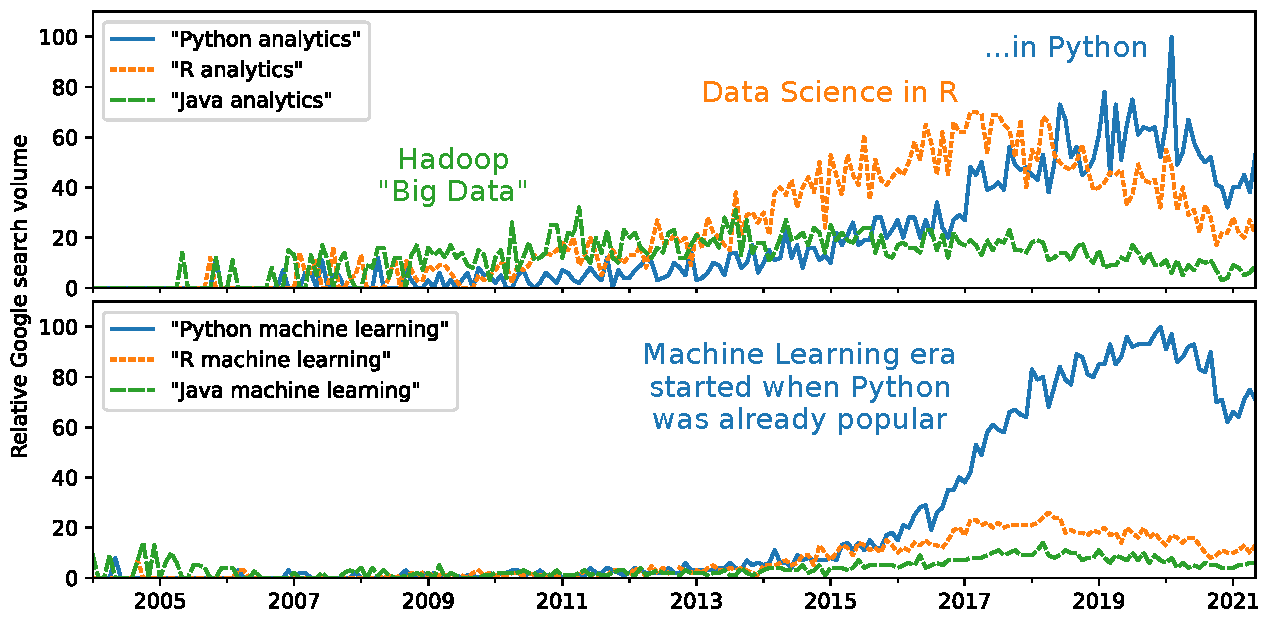
\includegraphics[width=\linewidth]{PLOTS/analytics-by-language.pdf}
\end{frame}

\begin{frame}{Python use has also been rising---steadily---in NHEP}
\vspace{0.15 cm}
\begin{columns}
\column{1.1\linewidth}
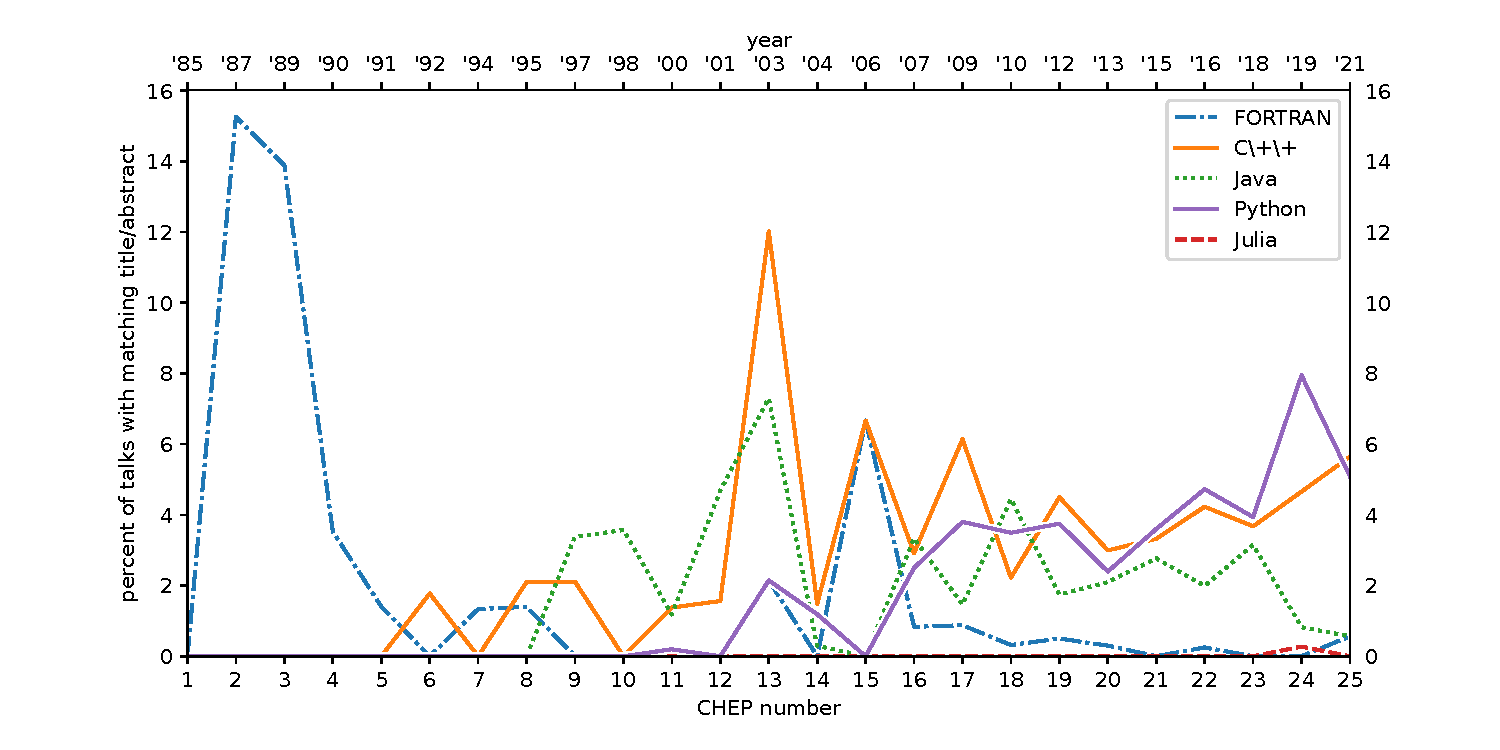
\includegraphics[width=\linewidth]{PLOTS/chep-papers-language-2.pdf}
\end{columns}
\end{frame}

\begin{frame}{Since {\it before} the return of machine learning}
\vspace{0.15 cm}
\begin{columns}
\column{1.1\linewidth}
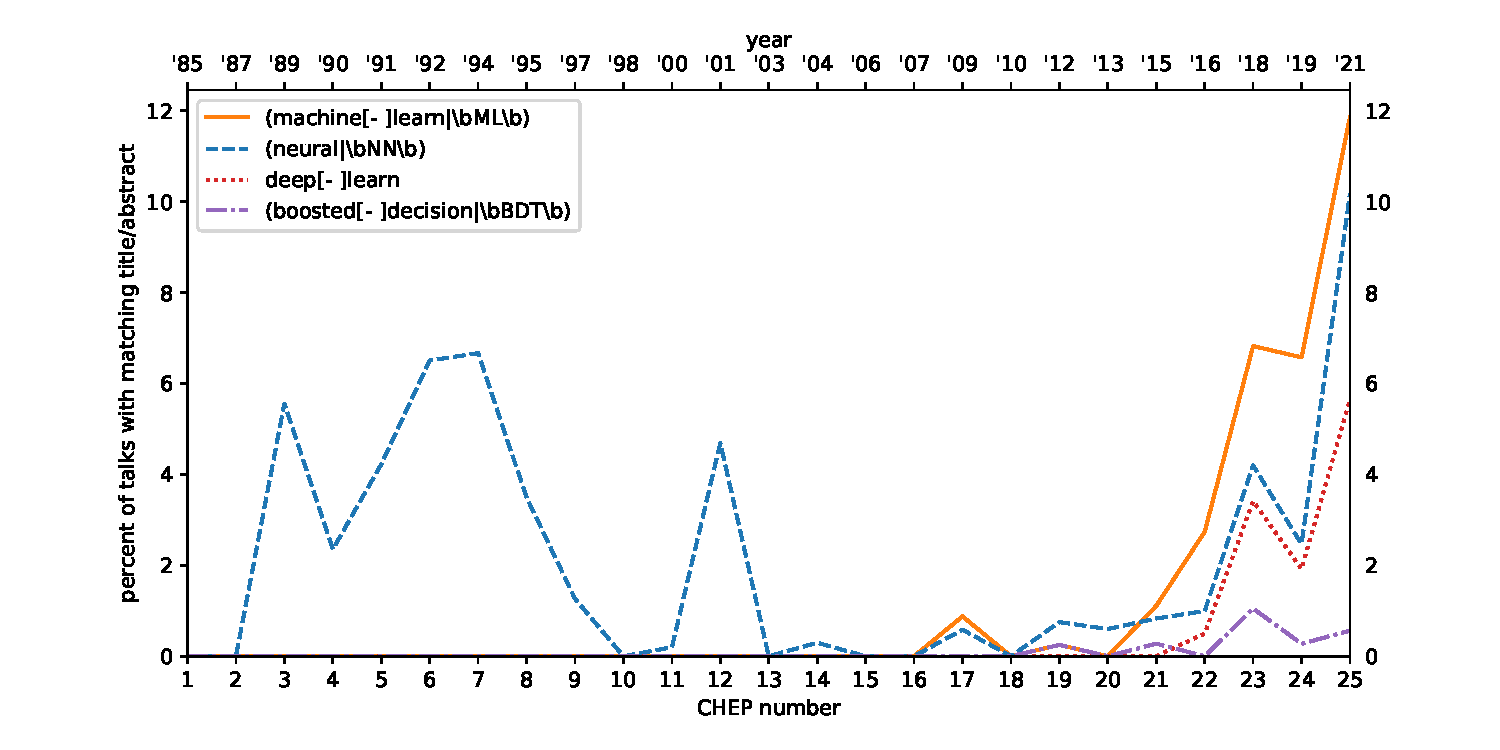
\includegraphics[width=\linewidth]{PLOTS/chep-papers-ml.pdf}
\end{columns}
\end{frame}

\begin{frame}{Lucas Taylor, {\it Summary of Data Analysis Track,} CHEP 2001}
\vspace{0.15 cm}
\begin{center}
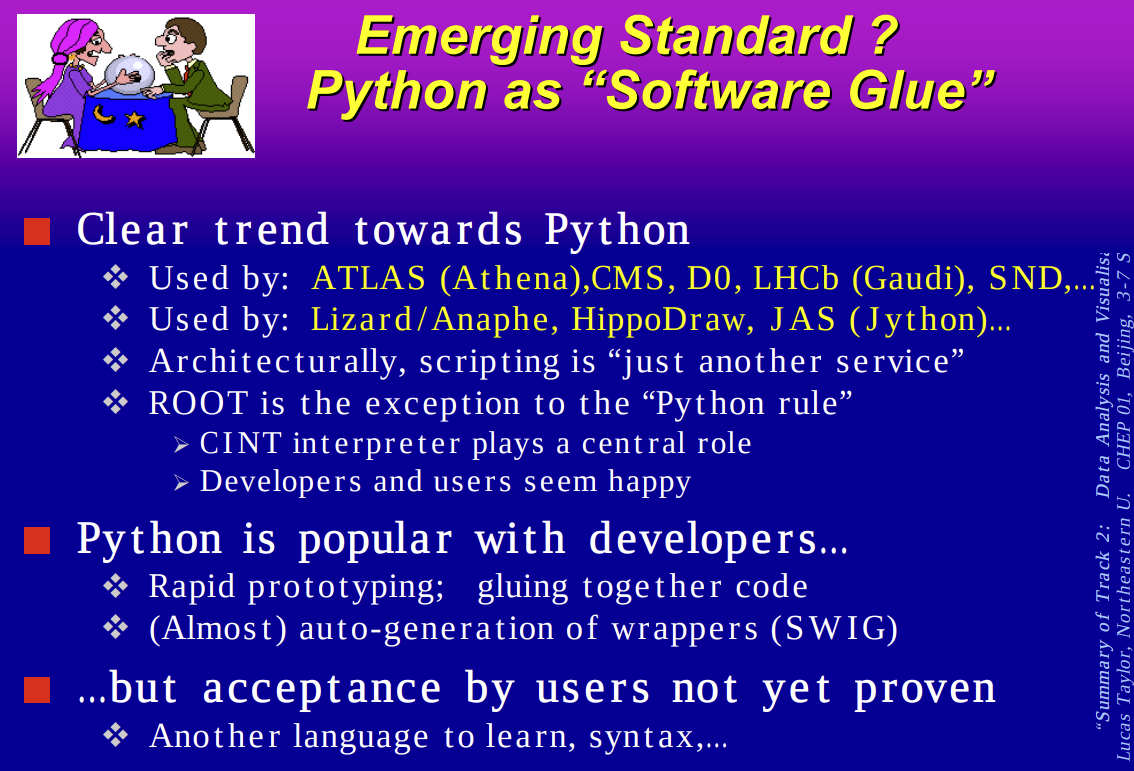
\includegraphics[width=0.81\linewidth]{PLOTS/chep-2001-python.png}
\end{center}
\end{frame}

\begin{frame}{Early adopters}
\vspace{0.5 cm}
\begin{columns}[t]
\column{0.52\linewidth}
Stephan Lammel, {\it Computing models of major HEP experiments: D\O\ and CDF}, 1997

\vspace{0.25 cm}
\includegraphics[width=\linewidth]{PLOTS/early-python-d0.png}

\column{0.45\linewidth}
Jeff Templon, {\it Python as an Integration Language}, SPAG-1998-02, 1998

\vspace{0.25 cm}
\includegraphics[width=\linewidth]{PLOTS/early-python-halla.png}

\end{columns}
\end{frame}






\end{document}
